% Emerson Ribeiro de Mello -- mello@sj.cefetsc.edu.br
% 2008-04-03
% ----------------------------------------------------------------------- %
% Modelo para monografia em LaTeX
%
% Este modelo faz uso da classe abntex para gerar um documento de acordo
% com a norma ABNT 14724 para apresenta��o de trabalhos acad�micos
%
% A classe abntex pode ser obtida em:
% http://abntex.codigolivre.org.br
%
% Arquivo: monografia.tex (principal)
% ----------------------------------------------------------------------- %

\documentclass[ruledheader]{abnt}

\usepackage{estilo-monografia}

\begin{document}

% inclus�o das partes iniciais do documento
% ----------------------------------------------------------------------- %
% Onde ser�o inseridas informa��es que ir�o aparecer na capa e na
% folha de rosto
%
% Arquivo: capa.tex
% ----------------------------------------------------------------------- %


\titulo{Plataforma para o Estudo de Mobilidade na Camada de Rede}

\autor{Cleiber Marques da Silva\\ Filipe Medeiros de Almeida}

\orientador{Prof. Eraldo Silveira e Silva}
% ou \orientador[Orientadora:\\]{Prof. Dra. Nome da orientadora}

%\coorientador{Nome do co-orientador}
% ou \coorientador[Co-orientadora:\\]{Prof. Dra. Nome da orientadora}

\comentario{Monografia apresentada � Coordena��o do Curso Superior de Tecnologia
em Sistemas de Telecomunica��es do Instituto Federal de Educa��o, Ci�ncia e
Tecnologia de Santa Catarina para a obten��o do diploma de Tecn�logo em Sistemas
de Telecomunica��es.}


\instituicao{Curso Superior de Tecnologia em Sistemas de Telecomunica��es \par 
	Instituto Federal de Educa��o, Ci�ncia e Tecnologia de Santa Catarina}

\local{S�o Jos� -- SC}

\data{Mar�o / 2009}

\capa

\folhaderosto

% ----------------------------------------------------------------------- %
% Onde ser�o inseridas informa��es que ir�o compor a folha de aprova��o
%
% Arquivo: folhadeaprovacao.tex
% ----------------------------------------------------------------------- %

\begin{folhadeaprovacao}
Monografia sob o t�tulo \textit{``Mobilidade em Redes IP: An�lise dos Protocolos MIPv6 e HMIPv6''}, defendida por Cleiber Marques da Silva e Filipe Medeiros de Almeida e aprovada em 06 de Mar�o de 2009, em S�o Jos�, Santa Catarina, pela banca examinadora assim constitu�da:

\setlength{\ABNTsignthickness}{0.4pt}
\setlength{\ABNTsignwidth}{10cm}
\setlength{\ABNTsignskip}{3.5cm}

\assinatura{Prof. Dr. Eraldo Silveira e Silva \\ Orientador}
\assinatura{Prof. Dr. Nome de Um Membro da Banca \\ CEFET / SC}
\assinatura{Prof. Dr. Nome de Outro Membro da Banca \\ Departamento de Automa��o e Sistemas - UFSC}

\end{folhadeaprovacao}

% ----------------------------------------------------------------------- %
% Pequena dedicat�ria ou uma ep�grafe (uma cita��o pertinente ao seu
% trabalho ou que represente o seu modo de pensar.)
% 
%
% Arquivo: dedicatoria.tex
% ----------------------------------------------------------------------- %

\vspace*{\fill}

{ \raggedleft


\textit{In a world without fences and walls \\
who needs Windows and Gates.}


}
% ----------------------------------------------------------------------- %
% Um pequeno texto para agradecer �queles que contribu�ram de maneira
% relevante � elabora��o do trabalho 
%
% Arquivo: agradecimentos.tex
% ----------------------------------------------------------------------- %

\chapter*{Agradecimentos}

Aos meus queridos pais e familiares, que nunca mediram esfor�os para que eu
pudesse atingir meus objetivos. Al�m do apoio, confian�a, dedica��o e presen�a
constante em todos os momentos da minha vida.

Aos meus amigos que ao longo dos �ltimos anos, trabalhei, aprendi, festejei,
troquei ideias. A estes quero agradecer de forma especial pelo incentivo,
apoio e amizade.

Ao professor Eraldo, pelos esclarecimentos das d�vidas, todos os coment�rios
sempre �teis, colobora��o e dedica��o. Al�m da prontid�o para me auxiliar em
todos os momentos durante a elabora��o deste trabalho.

\textbf{\textit{Cleiber Marques da Silva}}


\vspace{2cm}

Aos meus pais e familiares, pela base s�lida que sempre me deu for�a para 
encarar a vida de frente. Principalmente aos meus pais, por serem um exemplo de
for�a de vontade, mas, que acima de tudo, me ensinaram a percorrer meu pr�prio 
caminho.

Aos amigos com quem tive todo o prazer em trocar experi�ncias, tanto em quest�es
academicas quanto no amadurecimento como pessoa, sendo na nossa querida 
institui��o de tijolos � vista, nas nossas festas ou nos bares da regi�o.

A todos os professores que contribu�ram decisivamente para a minha, e nossa,
forma��o academica, profissional e pessoal. Em especial ao meu orientador 
professor Eraldo, por todo o conhecimento passado, pelas excelentes supervis�es,
orienta��o e por sempre acreditar no potencial dos alunos.

\textbf{\textit{Filipe Medeiros de Almeida}}

% ----------------------------------------------------------------------- %
% Pequeno texto que em poucas palavras consegue expressar o trabalho.
% O resumo deve ser concebido de forma tal que, uma pessoa ao ler o resumo
% possa entender sobre qual assunto este trabalho trata.
%
% Arquivo: resumo.tex
% ----------------------------------------------------------------------- %

\begin{resumo}
A investiga��o de tecnologias que possibilitam a mobilidade de terminais no
�mbito da Internet vem ganhando um grande espa�o na comunidade cient�fica. As
solu��es de mobilidade na camada de rede, tal como o IP M�vel e seus derivados,
apresentam-se como uma forma transparente e elegante de tratar o deslocamento de
um n� m�vel entre sub-redes. Neste trabalho descreve-se a implementa��o de uma
plataforma de testes baseada em m�quinas virtuais UML com fins facilitar os
estudos dos referidos protocolos, e a implementa��o de uma vers�o experimental
do IP M�vel Hier�rquico. Tamb�m s�o apresentados resultados sobre a efici�ncia e
funcionamento dos protocolos estudados, a partir de cen�rios de testes
realizados sobre a plataforma.

\textbf{Palavras-chave:} IP M�vel, IP M�vel Hier�rquico, IP M�vel para o Linux,
Linux Modo Usu�rio, Plataforma de Testes.
\end{resumo}

% ----------------------------------------------------------------------- %
% Tradu��o do resumo para a l�ngua inglesa.
% 
% 
%
% Arquivo: abstract.tex
% ----------------------------------------------------------------------- %

\begin{abstract}
The investigation of technologies that enable the mobility of terminals in
the Internet has gained a large space in the scientific community. The
solutions for mobility in the network layer, such as Mobile IPv6 and its
derivatives, appear as a transparent and elegant way to deal with the
displacement of a mobile node between subnets. This work describes the
implementation of a testing platform based on UML virtual machines with the
purpose of facilitating studies of these protocols, specifically the Mobile IPv6
and the Hierarchical Mobile IPv6. The lack of an updated code for the 
last one motivated an implementation of a experimental version of
the Hierarchical Mobile IP. As an additional contribution, it is discussed 
preliminary results on the operation and performance of the studied protocols,
extracted from test scenarios performed on the platform.

\textbf{Keywords:} Mobile IP, Mobile IP Hierarchical, Mobile IP for Linux,
User Mode Linux, Platform of tests.
\end{abstract}


% listas autom�ticas: sum�rio, lista de figuras e lista de tabelas
\tableofcontents
\listoffigures
\listoftables

% inclus�o dos cap�tulos
% ----------------------------------------------------------------------- %
% Arquivo: introducao.tex
% ----------------------------------------------------------------------- %

\chapter{Introdu��o}
\label{c_introducao}

\section{Motiva��o}
\label{ci_s_motivacao}

A utiliza��o de dispositivos m�veis para o acesso a Internet vem crescendo
acentuadamente nos �ltimos anos. As novas aplica��es multim�dias incentivam esta
expans�o, aliadas a uma variedade de novas tecnologias de acesso sem fio que
permitem suportar taxas de transmiss�o em n�veis relativamente altos. Algumas
destas tecnologias, consideradas como camada de enlace e f�sica do
ponto de vista da arquitetura TCP-IP, possuem mecanismos para o tratamento de
movimentos entre esta��es base, minimizando os efeitos destas opera��es para o
usu�rio.

Contudo, a utiliza��o de redes IP em situa��es de mobilidade pode impactar
consideravelmente as camadas superiores, independentemente da tecnologia de
acesso. Comunica��es em andamento podem ser interrompidas de forma brusca e
novas comunica��es podem ser inviabilizadas quando um terminal m�vel se
movimenta para uma nova subrede IP. Este fato adv�m do car�ter de
posicionamento topol�gico dos endere�amentos IP. Uma mudan�a de subrede
inviabiliza, a priori, a utiliza��o de um endere�o IP da rede de origem, dado
que os protocolos de roteamento subjacentes n�o podem atualizar as rotas em
tempo real, evidenciando um problema de escalabilidade.

Uma s�rie de propostas da IETF vem de encontro a este problema. Estas propostas
orbitam em torno do protocolo IP m�vel, nas vers�es 4 e 6. O estudo e teste
destes protocolos envolve, normalmente, arranjos relativamente complexos com
estruturas de rede sem fio al�m de entidades associadas aos protocolos de
mobilidade da camada de rede. Esta constata��o � um dos fatores primeiros que
motivaram o desenvolvimento deste trabalho.


\section{Objetivos}

O presente trabalho visa o desenvolvimento de uma plataforma para o estudo
de protocolos de mobilidade na camada de rede, em particular os protocolos
MIPv6 e HMIPv6.

Como especifica��es b�sicas desta plataforma pode-se enumerar:
\begin{itemize}
 \item a execu��o real dos protocolos, de forma que se possa configur�-los e
execut�-los de forma muito pr�xima de cen�rios reais;
\item facilidades de constru��o de cen�rios sem a necessidade de arranjos de
rede sem fio, reproduzindo, no entanto, os movimentos que impactam a camada de
rede;
\item pronta disponibilidade de ferramentas de medi��o, an�lise de tr�fego, bem
como protocolos de roteamento din�micos;
\end{itemize}


\section{Organiza��o do texto}
\label{ci_s_organizacao}

Este trabalho est� organizado da seguinte forma. O cap�tulo 2 resume os dois
protocolos de mobilidade de interesse: o protocolo IP m�vel vers�o 6, MIPv6 e
sua extens�o, o protocolo IP m�vel hier�rquico, HMIPv6. O cap�tulo 3 apresenta
a plataforma de mobilidade desenvolvida com apoio de m�quinas virtuais. Tendo
em vista que foram realizadas modifica��es em um c�digo aberto do MIPv6, para
que se comportasse tal como o HMIPv6, no cap�tulo 4 � apresentada uma vis�o
geral deste c�digo, bem como as modifica��es realizadas no mesmo para a
obten��o do HMIPv6. No cap�tulo 5 a plataforma de mobilidade � explorada para a
constru��o de alguns cen�rios de mobilidade com o MIPv6 e o HMIPv6. O cap�tulo
6 conclui e apresenta as perspectivas futuras de trabalhos usando a plataforma.
% ----------------------------------------------------------------------- %
% Arquivo: mipv6.tex
% ----------------------------------------------------------------------- %
\chapter{Vis�o geral do protocolo MIPv6}
\label{c_mipv6}
\section{Introdu��o}
Na internet, cada pacote associado ao um fluxo de pacotes entre pontos comunicantes, � encaminhado em fun��o do endere�o de IP destino. Cabe ao protocolo de camada de rede chamado \textit{Internet Protocol} (IP), escolher qual caminho o pacote deve seguir para chegar ao seu destinat�rio, em redes muito complexas como a \textit{Internet} alguns protocolos de roteamento auxiliam na descoberta da localiza��o dos destinos dinamicamente. Alguns exemplos de protocolos de roteamento s�o o \textit{Open Shortest Path First} (OSPF), \textit{Routing Information Protocol} (RIP) e \textit{Border Gateway Protocol} (BGP).

Os endere�os IP acabam definindo a localiza��o geogr�fica de um ponto de acesso, os protocolos atuais da \textit{Internet} assumem que o n� n�o muda seu endere�o IP durante uma comunica��o ou seja n�o troca o seu ponto de acesso.

Caso um n� mude seu ponto de acesso na \textit{Internet}, normalmente ele deve reconfigurar um novo endere�o IP e um roteador padr�o, se uma comunica��o estiver estabelecida quando o n� efetuar a mobilidade os protocolos de roteamento n�o ser�o mais capazes de entregar os pacotes corretamente. Para continuar sua comunica��o sua nova rota deve ser propagada para toda estrutura de roteamento da rede, obviamente esta alternativa � inaceit�vel, pois seria invi�vel fazer isso em uma rede como a \textit{Internet}.

Com a inten��o de permitir que n�s possam se movimentar para diferentes sub-redes e continuem sua comunica��o, foi proposto o protocolo IP M�vel que garante que os pacotes sejam roteados para os n�s m�veis. Existem duas varia��es para o IP M�vel uma para o IPv4 e outra para o IPv6.

O foco deste trabalho ser� na vers�o para o IPv6, pois o IPv6 possui algumas vantagens sobre o IPv4 como maior n�mero de endere�os, suporte nativo para seguran�a, possibilidade de auto-configura��o e suporte ao IP M�vel.

O protocolo IPv6 m�vel (MIPv6) tem por objetivo permitir que n�s IPv6 se desloquem entre sub-redes, com diferentes tecnologias de acesso como \textit{Ethernet} e \textit{Wireless LAN} e continuem suas comunica��es. Sem suporte ao MIPv6 todos os pacotes destinados ao n� m�vel quando ele estiver fora de sua rede origem ser�o perdidos.

O protocolo possibilita ao n� m�vel comunicar-se com outros n�s, m�veis ou est�ticos, ap�s mudar seu ponto de conex�o e ser alcan�ado pelo mesmo endere�o IP, tornando a mobilidade transparente para as camadas superiores a de rede.

\section{Terminologia do MIPv6}
Alguns termos definidos pelo MIPv6:

\begin{description}
\item[N� m�vel:] � o terminal de rede que pode trocar seu ponto de acesso a internet sem deixar de ser alcan��vel via seu endere�o domiciliar.
\item[Endere�o domiciliar:] � o endere�o est�tico associado ao n� m�vel na rede domiciliar.
\item[\textit{Link} domiciliar:] \textit{link} onde o prefixo de subrede do n� movel � definido.
\item[Link externo:] algum \textit{link} que n�o seja \textit{link} domiciliar do n� m�vel.
\item[\textit{Care-of-address}:] endere�o IP dado ao n� m�vel quando estiver em um \textit{link} externo, o prefixo da rede deste endere�o � o da rede externa.
\item[N� correspondente:] � o n� com quem o n� m�vel esta se correspondendo, pode ser m�vel ou fixo.
\item[Agente domiciliar:] � um roteador no \textit{link} domiciliar com quem o n� m�vel registra seu \textit{care-of-address} sempre que esta em um \textit{link} externo.
\item[Movimento:] � uma troca de ponto de acesso na Internet.
\item[\textit{Binding}:] � associa��o do endere�o domiciliar do n� m�vel com seu \textit{care-of-address}.
 \end{description}

\section{Funcionamento}
No contexto do MIPv6 um n� m�vel est� sempre acess�vel por um mesmo endere�o IP, independente de seu ponto de conex�o com a \textit{Internet}. Este endere�o � chamado de endere�o domiciliar e � o endere�o IPv6 fixo global do n� m�vel na sua rede de origem. Todos os n�s correspondentes se utilizam deste endere�o para se comunicar com o n� m�vel.

Enquanto um n� m�vel estiver fora de sua rede de origem ele ter� no m�nimo dois endere�os atribu�dos a sua interface de rede:
\begin{enumerate}
\item O endere�o domiciliar sempre permanente;
\item Um endere�o chamado de \textit{care-of-address}, que se refere a rede visitada. A cada nova rede ser� configurado um \textit{care-of-address}.
\end{enumerate}

O \textit{Care-of-address} pode ser obtido pelas formas convencionais do IPv6, ou seja, por \textit{stateless autoconfiguration}, no qual o endere�o � gerado por meio de informa��es divulgadas pelos roteadores das sub-redes, ou por \textit{stateful autoconfiguration}, onde o endere�o e outros par�metros de configura��o s�o providos diretamente de um servidor, por exemplo, os mecanismos DHCPv6 e PPPv6.

Na rede visitada, ap�s detectar o movimento e configurar seu \textit{care-of-address}, o n� m�vel envia uma mensagem icmp de \textit{Binding Update} para seu agente domiciliar, e este faz a associa��o de seu endere�o domiciliar com o seu \textit{care-of-address}. O agente domiciliar registra a mensagem em seu \textit{cache} e em resposta envia um \textit{Binding Acknowledgement}. Ent�o passa a atuar como um \textit{proxy} interceptando todos os pacotes com destino ao n� m�vel e enviando-os via t�nel. O n� m�vel pode tamb�m informar ao n� correspondente sua localiza��o. Neste caso, assim que o n� correspondente atualizar seu \textit{cache}, ele encaminhar� os pacotes diretamente ao n� m�vel.

Duas formas de comunica��o portanto podem ser realizadas entre o n� m�vel e o correspondente: no primeiro modo com tunelamento bidirecional, todos os pacotes s�o encaminhados via agente domiciliar. Neste caso os pacotes com origem no n� correspondente s�o roteados para o agente domiciliar e este envia ao n� m�vel via t�nel. Os pacotes enviados pelo n� m�vel, com destino ao n� correspondente s�o enviandos via t�nel ao agente domiciliar (t�nel reverso) e estes s�o roteados normalmente da rede domiciliar para o n� correspondente. O agente domiciliar utiliza \textit{proxy Neighbor Discovery} para interceptar os pacotes com destino ao n� m�vel. Neste modo o n� correspondente n�o precisa ter suporte ao MIPv6.

O segundo modo, mais eficiente, chamado de otimiza��o de roteamento. O n� m�vel tamb�m faz uma associa��o do seu \textit{care-of-address} com o n� correspondente e este pode come�ar a endere�ar os pacotes diretamente ao \textit{care-of-address}, eliminando assim o congestionamento e poss�veis falhas no \textit{link} entre o n� m�vel e o agente domiciliar.

A figura \ref{f_mipv6} permite observar de forma simplificada os dois modos de opera��o do protocolo MIPv6.

\begin{figure}[!htpb]
	\centering
	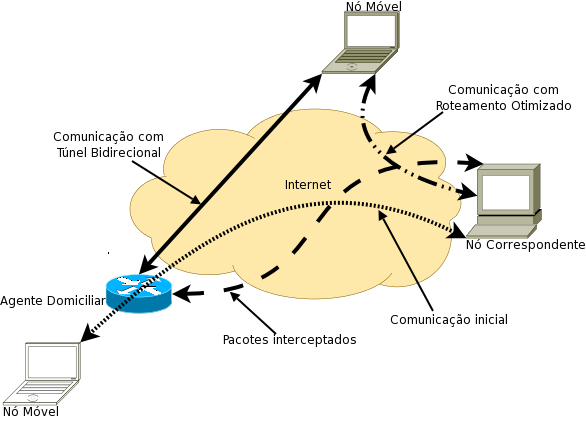
\includegraphics[scale=.5]{figs/mipv6}
 	\label{f_mipv6}
	\caption{Modos de opera��o simplificados do MIPv6}
\end{figure}

Enquanto estiver em uma rede visitada o n� m�vel ter�, portanto, mais de um endere�o configurado em sua interface, o endere�o domiciliar e um ou mais \textit{care-of-address}. Ele pode usar qualquer um desses endere�os para se comunicar. Com o intuito de manter a traspar�ncia para as camadas superiores � de rede o n� m�vel ir� utilizar geralmente seu endere�o domiciliar.

Ao enviar estes pacotes, eles dever�o ser modificados inserindo o \textit{care-of-address} no campo endere�o de origem e movendo o endere�o domiciliar para o campo \textit{home address}. No receptor do pacote estas altera��es devem ser revertidas para manter a transpar�ncia para as camadas superiores.

Uma das mais complicadas tarefas em mobilidade � o gerenciamento do \textit{handover} pelo n� m�vel. O gerenciamento do \textit{handover} pode se dar em diferentes camadas da arquitetura rede. O \textit{handover} de camada enlace refere-se a descoberta e conex�o h� uma nova rede. O \textit{handover} na camada rede �, no caso da arquitetura IPv6, envolve portanto:
\begin{enumerate}
 \item Descoberta de um novo roteador.
 \item Auto configura��o do \textit{care-of-address}.
 \item Teste de duplicidade do \textit{care-of-address} (DAD).
 \item Registro com o agente domiciliar e o n� correspondente.
\end{enumerate}

O in�cio de um handover de camada 3 se d� a partir de um mecanismo do protocolo IPv6 \textit{Neighbor Discovery}, incluindo os protocolos de \textit{Router Discovery} e \textit{Neighbor Unreachability Detection} para realizar esta detec��o.

Com o protocolo \textit{Neighbor Unreachability Detection} � poss�vel perceber que o roteador padr�o n�o est� mais alcan��vel, neste caso o n� deve descobrir um novo roteador padr�o.

O \textit{Router Discovery} � o protocolo que permite que n�s IPv6 descubram roteadores existentes no seu enlace, atrav�s das mensagens \textit{Router Advertisement} e \textit{Router Solicitation}. Um roteador IPv6 periodicamente envia mensagens de \textit{Router Advertisement} para todo o enlace, desta forma os n�s podem configurar seu endere�o de rede (\textit{stateless autoconfiguration})e roteadores padr�o. O n� tamb�m pode enviar uma mensagem de \textit{Router Solicitation} recebendo como resposta um \textit{Router Advertisement}.

Desta forma o n� m�vel pode perceber o movimento quando receber um \textit{Router Advertisement} de um novo roteador ou quando perceber que seu roteador n�o esta mais alcan��vel, ent�o deve requisitar um novo. Por meio das mensagens trocadas na descoberta do novo roteador o n� m�vel � capaz de gerar seu \textit{care-of-address}, ent�o o teste de duplicidade deve ser feito para verificar se n�o h� um endere�o igual no \textit{link}, com sucesso o registro com o agente domiciliar e o n� correspondente deve ser efetuado finalizando o processo de \textit{handover}.

\section{Mensagens do IPv6}
Ao detectar que n�o esta em sua rede domiciliar o n� m�vel deve enviar um \textit{Binding Update} ao seu home agente para informar o seu \textit{care-of-address}. No pacote de \textit{Binding Update} os seguintes requisitos devem ser seguidos:
\begin{itemize}
 \item bit H (\textit{home registration}) deve estar ligado;
 \item bit A (\textit{acknowledge}) deve estar ligado;
 \item o pacote deve ter a op��o de agente domiciliar preenchida;
 \item  endere�o de origem do pacote deve ser o \textit{care-of-address} a ser registrado, a menos
que a sub-op��o de \textit{care-of-address} alternativo esteja sendo utilizada;
 \item o tempo de vida do \textit{binding} deve ser menor ou igual ao do \textit{care-of-address}. 
\end{itemize}

Quando o n� m�vel retornar a sua rede de origem deve enviar um \textit{Binding Update} para o seu agente domiciliar, para que este pare de interceptar e tunelar os pacotes destinados a ele.

As mensagens de \textit{Binding Updates} trocadas nos dois modos de opera��o do MIPv6 podem ser observadas na figura \ref{f_messages}.

\section{Considera��es sobre Seguran�a}
O uso de \textit{Binding Updates} n�o autenticados � tido como um s�rio problema de seguran�a, pois, um n� mal intencionado pode forjar um registro com o n� correspondente e passar a receber os pacotes destinados ao n� m�vel. Com a inten��o de solucionar este problema de seguran�a, o protocolo MIPv6 implementa alguns mecanismos.

Para dar mais prote��o no processo de \textit{Binding Update} com o agente domiciliar pode se utilizar o protocolo IPsec nativo no IPv6. A troca de mensagens pode ser feita utilizando o protocolo AH do IPsec. Para isto � necess�rio um relacionamento pr�vio de seguran�a entre o n� m�vel e o agente domiciliar, ou seja, uma chave secreta deve ser configurada nos dois n�s.

No processo do registro do n� m�vel com o n� correspondente torna-se imposs�vel utilizar o IPsec para prover seguran�a no processo, pois o n� correspondente pode ser estar localizado em qualquer lugar na \textit{Internet} e uma chave secreta n�o pode ser pr�-configurada. Para tornar o processo seguro faz-se necess�rio o uso de algum mecanismo global de autentica��o autom�tica. A solu��o proposta para esse problema � conhecida como \textit{Return Routability Procedure}. 

\subsection{\textit{Return Routability Procedure}}
Na tentativa de tornar mais seguro o registro do n� m�vel com o n� correspondente o MIPv6 introduz uma solu��o bastante inteligente: o \textit{Return Routability Procedure}. A id�ia do processo � que o n� correspondente obtenha garantias de que o n� m�vel seja alcan��vel pelo seu endere�o domiciliar e o \textit{care-of-address}. Somente assim o n� correspondente estar� apto para receber \textit{Binding Updates}.

O teste consiste em enviar, a partir do n� m�vel, duas mensagens ao n� correspondente uma via agente domiciliar (\textit{Home Test Init}) e outra diretamente ao n� correspondente (\textit{Care-of Test Init}). Em resposta o n� correspondente envia duas mensagens (\textit{Home Test} e \textit{Care-of Test}). A partir dos dados destas mensagens o n� m�vel � capaz de gerar uma chave de seguran�a denominada \textit{binding management key} (Kbm).

Na figura \ref{f_messages} pode-se observar o fluxo das mensagens utilizados no \textit{Return Routability Procedure}.
\begin{figure}[!htpb]
	\centering
	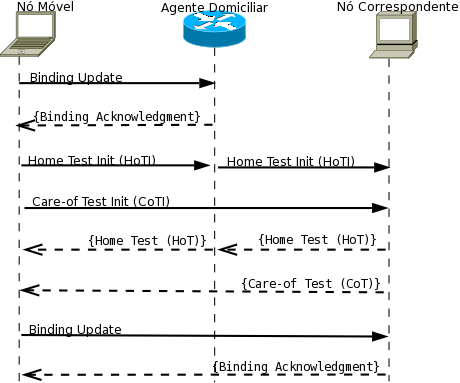
\includegraphics[scale=.5]{figs/messages}
 	\label{f_messages}
	\caption{Mensagens MIPv6}
\end{figure}

Para autorizar o \textit{Binding Update} o n� m�vel gerou a Kbm que permite uma verifica��o por parte do n� correspondente. Ao receber o \textit{Binding Update} o n� correspondente � capaz de recalcular a Kbm e permitir a associa��o do \textit{care-of-address} com o endere�o domiciliar.

� importante salientar que o \textit{Return Routability Procedure} n�o � totalmente seguro, pois um atacante pode capturar as mensagens enviadas pelo n� correspondente e forjar mensagens de \textit{Binding Updates}. Obviamente o mesmo atacante conseguir� fazer o mesmo ataque em uma rede IPv6 sem mobilidade. Podemos concluir que o \textit{Return Routability Procedure} n�o introduz riscos adicionais ao protocolo IPv6 b�sico. 

% ----------------------------------------------------------------------- %
% Arquivo: simulacao.tex
% ----------------------------------------------------------------------- 

\chapter{Plataforma de Testes}
\label{c_simulacao}
O objetivo deste cap�tulo � descrever todos os procedimentos efetuados para montar um ambiente de simula��o, que ir� auxiliar na an�lise do protocolo MIPv6, vamos usar simula��o devido a facilidade e rapidez para constru��o dos cen�rios, al�m disso realizar os experimentos fisicamente envolvem um alto custo e demandam muito tempo. No ambiente simula��o faremos o uso da m�quina virtual \textit{User Mode Linux} (UML), pois � incorporada ao kernel e apresenta um alto desempenho em execu��o.

Nos testes envolvendo o protocolo � necess�rio um Kernel Linux compilado com suporte ao MIPv6, uma instala��o do \textit{Mobile IPv6 for Linux} (MIPL) uma implementa��o do IPv6 M�vel para o Linux, e a instala��o do \textit{Router ADVertisement Daemon} (RADVD) necess�rio em redes IPv6 para gerar \textit{router advertisement} e escutar \textit{router solicitations}.

\section{UML}
\label{s_uml}
UML (\textit{User Mode Linux}) � uma m�quina virtual para sistemas Linux, � uma implementa��o que permite que o Kernel Linux rode no sistema operacional Linux como um processo normal, diferente de outras tecnologias de virtualiza��o que emulam uma plataforma f�sica. Com UML � poss�vel criar m�quinas virtuais para ajudar no desenvolvimento de aplica��es, servi�os de rede, implementa��o clusters de rede, testes de seguran�a.

Para utilizar uma m�quina virtual UML somente � necess�rio uma vers�o do Kernel Linux compilado para a arquitetura UML e um sistema de arquivos. No endere�o http://uml.nagafix.co.uk/ h� dispon�vel v�rios sistemas de arquivos, no ambiente de simula��o utilizaremos um baseado no Linux Debian. Para iniciar a constru��o do ambiente de simula��o vamos fazer o download do sistema de arquivos:

\begin{verbatim}
 # mkdir vm
 # cd vm
 # wget http://uml.nagafix.co.uk/Debian-4.0/Debian-4.0-x86-root_fs.bz2
 # bunzip2 Debian-4.0-x86-root_fs.bz2
 # mv Debian-4.0-x86-root_fs DebianFS
\end{verbatim}

Um pacote de ferramentas para UML chamado \textit{uml\_utilities} deve ser instalado no sistema hospedeiro para permitir interligar as m�quinas virtuais em rede, e auxiliar no ambiente de testes.

\begin{verbatim}
 # wget http://prdownloads.sourceforge.net/user-mode-linux\
 /uml_utilities_20040406.tar.bz2
 # tar jxvf uml_utilities_20040406.tar.bz2 && cd tools
 # make && make install 
\end{verbatim}

O \textit{uml\_switch} que acompanha este pacote n�o permite a simula��o de mobilidade, algumas altera��es no c�digo do \textit{uml\_switch} foram feitas pelo desenvolvedor do projeto "Avalia��o do Protocolo Fast Handover MIPv6" que permitem a simula��o da mobilidade. Ser� preciso desta vers�o para o ambiente:

\begin{verbatim}
 # wget http://algum.lugar
 # tar xvzf uml_switch.tar.gz && cd uml_switch
 # make && make install
\end{verbatim}

\section{Kernel}
\label{s_kernel}
Para o ambiente de simula��o precisamos um kernel compilado para a arquitetura UML com suporte a MIPv6. No kernel o suporte nativo do protocolo MIPv6 est� dispon�vel desde a vers�o 2.6.17, nestes cen�rios de testes ser� utilizado a vers�o 2.6.25.6 do kernel. Para iniciar o trabalho de compila��o � necess�rio fazer o download dos c�digos fontes do kernel:
\begin{verbatim}
 # wget http://kernel.org/pub/linux/kernel/v2.6/linux-2.6.25.6.tar.bz2
 # tar jxvf linux-2.6.25.6.tar.bz2
 # cd linux-2.6.22.6
\end{verbatim}

Configurando a arquitetura na qual o kernel ser� compilado:
\begin{verbatim}
 # export ARCH=um
\end{verbatim}

Configurando o kernel:
\begin{verbatim}
 # make defconfig
 # make menuconfig
\end{verbatim} 

� interessante habilitar a op��o HOSTFS para as m�quinas virtuais terem acesso ao sistema de arquivos do hospedeiro.
\begin{verbatim}
 UML-specific options
-->Host filesystem [HOSTFS]
\end{verbatim}

Para configurar o kernel com suporte ao MIPv6 estas s�o as op��es m�nimas que devem ser setadas:
\begin{verbatim}
 CONFIG_EXPERIMENTAL=y
 CONFIG_SYSVIPC=y
 CONFIG_PROC_FS=y
 CONFIG_NET=y
 CONFIG_INET=y 
 CONFIG_IPV6=y
 CONFIG_IPV6_MIP6=y
 CONFIG_XFRM=y
 CONFIG_XFRM_USER=y
 CONFIG_XFRM_SUB_POLICY=y
 CONFIG_INET6_XFRM_MODE_ROUTEOPTIMIZATION=y
\end{verbatim}

Op��es que o agente domiciliar e o n� m�vel necessitam:
\begin{verbatim}
 CONFIG_IPV6_TUNNEL=y
 CONFIG_IPV6_MULTIPLE_TABLES=y
\end{verbatim}

Op��o que o n� m�vel tamb�m necessita:
\begin{verbatim}
 CONFIG_IPV6_SUBTREES=y
\end{verbatim}

Para alguns indicadores de movimento do n� m�vel, pode ser setado:
\begin{verbatim}
 CONFIG_ARPD=y
\end{verbatim}

Para suporte ao IPsec � necess�rio pelo menos:
\begin{verbatim}
 CONFIG_INET6_ESP=y
\end{verbatim}

Para utilizar IPsec nos t�neis:
\begin{verbatim}
 CONFIG_NET_KEY=y
 CONFIG_NET_KEY_MIGRATE=y
\end{verbatim}

No menu de configura��o estas s�o as op��es que devem ser setadas:
\begin{verbatim}
Code maturity level options
--> Prompt for development and/or incomplete code/drivers [CONFIG_EXPERIMENTAL]

General setup 
--> System V IPC [CONFIG_SYSVIPC]

Networking
--> Networking support [CONFIG_NET]
--> Networking options
    --> Transformation user configuration interface [CONFIG_XFRM_USER]
    --> Transformation sub policy support [CONFIG_XFRM_SUB_POLICY]
    --> Transformation migrate database [CONFIG_XFRM_MIGRATE]
    --> PF_KEY sockets [CONFIG_NET_KEY]
    --> PF_KEY MIGRATE [CONFIG_NET_KEY_MIGRATE]
    --> TCP/IP networking [CONFIG_INET]
    --> The IPv6 protocol [CONFIG_IPV6]
    --> IPv6: AH transformation [CONFIG_INET6_AH]
    --> IPv6: ESP transformation [CONFIG_INET6_ESP]
    --> IPv6: IPComp transformation [CONFIG_INET6_IPCOMP]
    --> IPv6: Mobility [CONFIG_IPV6_MIP6]
    --> IPv6: IPsec transport mode [CONFIG_INET6_XFRM_MODE_TRANSPORT]
    --> IPv6: IPsec tunnel mode [CONFIG_INET6_XFRM_MODE_TUNNEL]
    --> IPv6: MIPv6 route optimization mode [XFRM_MODE_ROUTEOPTIMIZATION]
    --> IPv6: IPv6-in-IPv6 tunnel [CONFIG_IPV6_TUNNEL]
    --> IPv6: Multiple Routing Tables [CONFIG_IPV6_MULTIPLE_TABLES]
    --> IPv6: source address based routing [CONFIG_IPV6_SUBTREES]
File systems
--> Pseudo filesystems
    --> /proc file system support [CONFIG_PROC_FS]
\end{verbatim}

Para verificar se o kernel est� configurado corretamente para MIPv6 existe o \textit{shell script} \textbf{\textit{chkconf\_kernel.sh}} que acompanha o pacote do MIPL.

Ap�s a configura��o o kernel vamos compil�-lo e os seus m�dulos devem ser copiados para o sistema de arquivos, por isso ser�o instalados no diret�rio uml-modules para depois serem copiados.
\begin{verbatim}
 # make
 # strip linux
 # make modules_install INSTALL_MOD_PATH=uml-modules
 # unset arch
\end{verbatim}

Para copiar os m�dulos do kernel para o sistema de arquivos:
\begin{verbatim}
# cd ..
# mkdir loop
# mount -o loop DebianFS loop
# cp -rf linux-2.6.25.6/uml-modules/lib/modules/* loop/lib/modules
\end{verbatim}

� preciso copiar os arquivos fontes do kernel para o sistema de arquivos, pois o MIPL vai precisar para a sua compila��o.
\begin{verbatim}
# cp -r linux-2.6.25.6.tar.bz2 loop/usr/src/
# cd loop/usr/src
# tar jxvf linux-2.6.25.6.tar.bz2
# ln -s linux-2.6.25.6 linux
# rm linux-2.6.25.6.tar.bz2
# cd ../../../
# umount loop
\end{verbatim}

\section{Preparando o sistema de arquivos}
\label{s_prep}
Alguns pacotes de desenvolvimento, bibliotecas dever�o ser instalados no sistema de arquivos, pois os programas MIPL e RADVD ser�o compilados na m�quina virtual. E para auxiliar na analise dos cen�rios ser�o instaladas algumas ferramentas de rede.

Para poder fazer o download dos pacotes � necess�rio a cria��o de uma rede entre o hospedeiro e a m�quina virtual. Neste caso deve-se criar uma interface virtual no hospedeiro, o m�dulo \textbf{\textit{tun}} deve estar carregado no sistema.
\begin{verbatim}
 # modprobe tun
 # tunctl -u <nome do usu�rio>
\end{verbatim}

Configurando a interface virtual do hospedeiro, habilitando o roteamento de pacotes e o nat para os pacotes da m�quina virtual:
\begin{verbatim}
# ifconfig tap0 192.168.1.1 netmask 255.255.255.0
# echo 1 > /proc/sys/net/ipv4/ip_forward
# iptables -t nat -I POSTROUTING -o eth0 -j MASQUERADE
# iptables -I FORWARD -i tap0 -j ACCEPT
# iptables -I FORWARD -o tap0 -j ACCEPT
\end{verbatim}

Iniciando a m�quina virtual, para se logar use \textit{root} sem senha:
\begin{verbatim}
 # cp linux-2.6.25.6/linux .
 # ./linux ubda=DebianFS mem=128M eth0=tuntap,tap0
\end{verbatim}

Configurando a rede na maquina virtual:
\begin{verbatim}
 uml# ifconfig eth0 192.168.1.2 netmask 255.255.255.0
 uml# route add default gw 192.168.1.1
 uml# echo nameserver <seu_dns> > /etc/resolv.conf
\end{verbatim}

Na distribui��o Linux Debian h� um gerenciador de pacotes o \textbf{\textit{apt}} que facilita a instala��o de programas, ele permite procurar e instalar pacotes. Para utilizar � necess�rio configurar um reposit�rio de pacotes:
\begin{verbatim}
 uml# echo deb http://security.debian.org/ etch/updates main contrib > \
 /etc/apt/source.list
\end{verbatim}

Os seguinte pacotes ser�o instalados:
\begin{itemize}
 \item gcc-4.1
 \item libc6-dev
 \item make
 \item libtool
 \item automake1.9
 \item autoconf2.13
 \item bison
 \item patch
 \item flex
 \item indent
 \item telnet
 \item tcpdump
 \item tethereal
 \item iproute
 \item subversion
\end{itemize}

Para instalar utilizando o \textbf{\textit{apt}}:
\begin{verbatim}
 uml# apt-get update
 uml# apt-get install gcc-4.1 libc6-dev make libtool automake1.9 \
 autoconf2.13 bison patch flex indent telnet tcpdump tethereal  \
 iproute subversion
\end{verbatim}

\section{MIPL}
\label{s_mipl}
O MIPL (\textit{Mobile IPv6 for Linux}) � uma implementa��o de Suporte a Mobilidade no IPv6 (RFC 3775), desenvolvida na Universidade Tecn�logica de Helsinki. � um programa em \textit{user space} que trabalha junto com MIPv6 habilitado no kernel.

Vamos fazer o download da ultima vers�o est�vel do MIPL:
\begin{verbatim}
 uml# wget ftp://ftp.linux-ipv6.org/pub/usagi/patch/mipv6/umip-0.4/daemon\
 /tarball/mipv6-daemon-umip-0.4.tar.gz
 uml# tar xvzf mipv6-daemon-umip-0.4.tar.gz && cd mipv6-daemon-umip-0.4
\end{verbatim}

Vamos configurar o MIPL para buscar os cabe�alhos do kernel no local onde foram copiados, habilitaremos a compila��o de um virtual terminal onde poderemos acessar para acompanhar o protocolo em execu��o.

\begin{verbatim}
 uml# CPPFLAGS='-isystem /usr/src/linux/include' ./configure --enable-vt 
\end{verbatim}

Compilando e instalando:
\begin{verbatim}
 uml# make
 uml# make install
\end{verbatim}

\subsection{Configurando MIPL}
Nesta se��o pretende-se mostrar como configurar o \textit{daemon} do MIPL para rodar como um n� m�vel, um agente domicili ou um n� correspondente, explanando todas as op��es do seu arquivo de configura��o.

Esta s�o as op��es comuns ao n� m�vel, ao agente domiciliar e ao n� corresponde do arquivo de configura��o do MIPL.
\subsubsection{NodeConfig CN | HA | MN;}
Indica se o \textit{daemon} deve rodar como n� correposdente, agente domiciliar ou n� m�vel. A configura��o padr�o � CN.
\subsubsection{DebugLevel number;}
Indica ao \textit{daemon} o nivel de \textit{debug}, se o valor for maior que zero, o \textit{daemon} ir� imprimir mensagens de \textit{debug} no console. A configura��o padrao � 0.
\subsubsection{DoRouteOptimizationCN boolean;}
Indica se o n� deve participar da otimiza��o de roteamento com o n� m�vel. A configura��o padr�o � habilitado.

Op��es comuns ao n� m�vel e ao agente domiciliar:
Falta explicar v�rios par�metros ainda.

\section{RADVD}
\label{s_radvd}
O RADVD (\textit{Router ADVertisement Daemon})� um servi�o para roteadores IPv6. Ele envia mensagens \textit{Router Advertisement} e responde a \textit{Router Solicitation} especificadas na RFC 2641. Essas mensagens s�o utilizadas para \textit{stateless autoconfiguration}. Vamos fazer o download do pacote, compilar e instalar:

\begin{verbatim}
 uml# wget http://www.litech.org/radvd/dist/radvd-1.1.tar.gz
 uml# tar xvzf radvd-1.1.tar.gz && cd radvd-1.1
 uml# make && make install
\end{verbatim}

\subsection{Configurando RADVD}
Op��es do arquivo de configura��o ...

\section{Gerador de tr�fego}
\label{s_trafego}
Para auxiliar nos testes do protocolo MIPv6 foi criado uma simples aplica��o chamada \textbf{\textit{gen}} que permite gerar trafegos TCP e UDP na rede. O programa foi desenvolvido utilizando a linguagem C e a API de \textit{sockets}, � semelhante a ferramenta \textit{ping}, por�m utiliza as camadas de aplica��o e de transporte. Com o \textbf{\textit{gen}} permite-se observar a transpar�ncia do protocolo com as camadas superiores a de rede.

Vamos fazer o download do programa e sua compila��o:
\begin{verbatim}
uml# wget http://
uml# gcc -o gen gen.c
uml# mv gen /bin
\end{verbatim}

Para utilizar o programa, � preciso que um n� da rede inicie o gen e fique esperando pacotes, desta forma:
\begin{verbatim}
 mn# gen
\end{verbatim}

E outro n� deve iniciar o gen passando como par�metro o endere�o IP do outro n�, desta forma:
\begin{verbatim}
 cn# gen 2000:a::1
\end{verbatim}
% ----------------------------------------------------------------------- %
% Arquivo: cenarios.tex
% ----------------------------------------------------------------------- %

\chapter{Cen�rios de Testes}

\section{Introdu��o}
Ap�s os estudos bibliogr�ficos sobre o protocolo MIPv6 e a prepara��o da Plataforma
 de Testes para Mobilidade, iniciou-se a etapa de defini��o e implementa��o de cen�rios
 com fins de analisar as funcionalidade dos protocolos.

Para analisar alguns mecanismos do protocolo e testar seus modos de opera��o, dois 
 cen�rios base foram definidos. Nesses dois cen�rios foi realizada tr�s simula��es.
 A primeira simula��o ocorre no cen�rio 1, descrito na figura \ref{f_cenario1}, onde
 � testado o modo de opera��o por tunelamento bi-direcional do MIPv6. A segunda simula��o
 tambem ocorre no cen�rio 1, sendo testado o modo de opera��o por otimiza��o de roteamento
 A terceira simula��o � no cen�rio 2, descrito na figura\ref{f_cenario2}, tendo como
 objetivo o funcionamento do HMIPv6.

%O computador que ser� utilizado para a realiza��o dos cen�rios de teste possui as seguintes 
% caracteristicas: \textit{Atlhon XP 2600}, 512MB de mem�ria e rodando \textit{Gnu/Linux 
% Slackware} 12.0, kernel linux-2.6.21.5.

Os arquivos para a configura��o dos cen�rios usados no Guml4Mip est�o dispon�veis no
 diret�rio da documenta��o do projeto.

%Para auxiliar na gera��o de \textit{logs}, que tendem a enriquecer an�lise dos cen�rios, foram utilizadas as ferramentas
%\textit{tcpdump}, \textit{ping6} e \textit{gen}.

\section{Fundamentos para a An�lise dos Cen�rios}
  Na an�lise dos cen�rios estudados vamos localizar os seguintes aspectos:
\begin{itemize}
  \item a sequ�ncia e a natureza das mensagens trocadas entre os v�rios n�s. Neste
 aspecto, utilizaremos as sa�das geradas pelos programas \textit{tcpdump};
  \item as tabelas de roteamento e regras de roteamento analisadas em situa��es chave,
 por exemplo, antes e depois da mobilidade;
  \item aspectos de desempenho e perdas de pacotes. Sabemos das limita��es desta an�lise 
 em um ambiente virtual, mas esperamos obter dados relativos. Tamb�m confrontaremos os dados
 obtidos com os resultados esperados segundo uma abordagem anal�tica.
  \item A cria��o e a manipula��o dos tuneis entre o agente domiciliar e o n� m�vel antes
 e depois do movimento.
\end{itemize}

\subsection{Tempo de lat�ncia do \textit{Handover}}
O processo de \textit{handover} acontece quando o n� m�vel muda seu ponto de conex�o 
 de uma sub-rede para outra. O tempo de lat�ncia envolvido neste processo \cite{xavier}
 pode ser dividida em quatro fases:

\begin{enumerate}
 \item \textbf{Detec��o de Movimento (\textit{TD})}: Em um cen�rio real representaria
 o tempo do \textit{handover} na camada de enlace at� o primeiro \textit{Router Advertisement}.
 Como neste ambiente de testes n�o conseguimos simular a camada enlace n�o se pode precisar
 com a exatid�o a lat�ncia envolvida no processo. Por�m, para fins de estudo consideraremos
 para nosso cen�rio o tempo entre o �tlimo pacote do \textit{gen} recebido na rede
 domiciliar e o primeiro \textit{Router Advertisement} na rede visitada.

\begin{equation}
 TD = t1 - t0
\label{eq.td}
\end{equation}

\item \textbf{Configura��o do \textit{Care-of-address} (\textit{TA})}: Tempo que entre 
 o primeiro \textit{Router Advertisement} e o envio do \textit{Binding Update}.

\begin{equation}
 TA = t2 -t1
 \label{eq.ta}
\end{equation}

\item \textbf{Registro com agente domiciliar (\textit{TR})}: Intervalo de tempo entre
 o envio do \textit{Binding Update} ao agente domiciliar e o recebimento do
 \textit{Binding Acknowledgement}.

\begin{equation}
 TR = t3 - t2
 \label{eq.tr}
\end{equation}

\item \textbf{Otimiza��o de Roteamento (\textit{TO})}: Intervalo de tempo entre o envio
 das mensagens do \textit{Return Routability Procedure} e o recebimento do
 \textit{Binding Acknowledgement} do n� correspondente.

\begin{equation}
 TO = t4 - t3
 \label{eq.to}
\end{equation}

\end{enumerate}

Obviamente podemos calcular o tempo de lat�ncia do handover com a seguinte f�rmula:

\begin{equation}
 TH = TD + TA + TR + TO
 \label{eq.th}
\end{equation}

\section{Cen�rio 1}
\label{s_cenario1}
O primeiro cen�rio de teste � formado por tr�s redes interligadas entre si e cinco n�s. A sua topologia pode ser observada na figura \ref{f_cenario1}, onde o numero nos bal�es cinza representam a vlan no \textit{uml-switch}. Os endere�os atribu�dos as interfaces dos n�s, durante a realiza��o do cen�rio, bem como seus endere�os de hardware est�o dispon�veis na tabela \ref{t_addr1}.

\begin{figure}[!htpb]
	\centering
	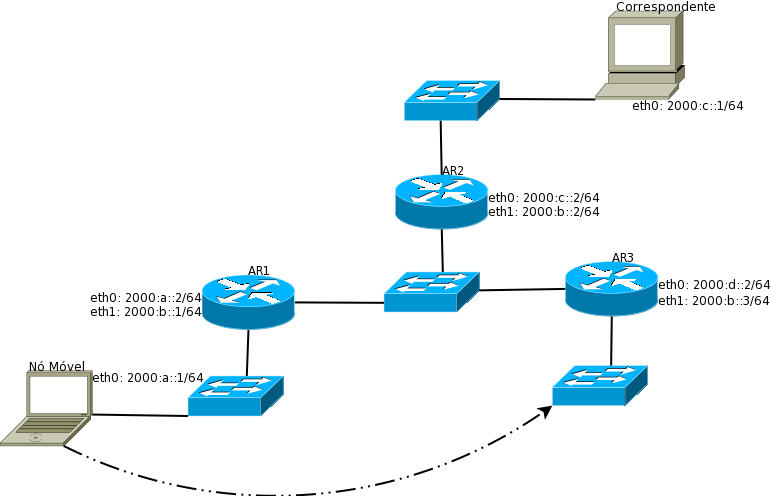
\includegraphics[scale=.4]{figs/cenario1}
	\caption{Topologia do Cen�rio 1}
	\label{f_cenario1}
\end{figure}


Na rede com prefixo 2000:a::/64 est� o n� correspondente com quem o n� m�vel est� se comunicando. Na rede com o prefixo
 2000:c::/64 est� presente um roteador (HA) que oferece o servi�o de agente domiciliar ao n� m�vel. A rede com prefixo
 2000:d::/64 � a rede que o n� m�vel deve visitar.

\begin{table}[!htpb]
\centering
\begin{small}
  \setlength{\tabcolsep}{3pt}
\begin{tabular}{|c|c|c|c|c|}\hline
\raisebox{1.5ex}{N�} & \raisebox{1.5ex}{Interface} & \raisebox{1.5ex}{MAC} & \raisebox{1.5ex}{Endere�o} & \raisebox{1.5ex}{Tipo}\\ \hline
% MN
& & & 2000:a::1 & Domiciliar (Global) \\ 
MN & eth0 & 92:09:4F:D5:EF:EA & 2000:a::9009:4fff:fed5:efea & Auto-configurado \\
& & & 2000:d::9009:4fff:fed5:efea & Care-of-address \\
& & & fe80::9009:4fff:fed5:efea & Local \\ \hline
% CN
CN & eth0 & D6:7F:B0:C3:C9:0C & 2000:c::1 & Global \\ 
& & & fe80::d47f:b0ff:fec3:c90 & Local \\ \hline
% AR1
& eth0 & AE:4D:A8:10:EB:1D & 2000:a::2 & Global \\ 
AR1 & & & fe80::ac4d:a8ff:fe10:eb1d & Local \\
& eth1 & 1E:2D:C8:43:E6:C7 & 2000:b::1 & Global \\ 
& & & fe80::1c2d:c8ff:fe43:e6c7 & Local \\ \hline
%AR2
& eth0 & 36:A7:3F:06:58:8D & 2000:c::2 & Global \\ 
AR2 & & & fe80::34a7:3fff:fe06:588d & Local \\ 
& eth1 & 4A:19:FD:12:48:34 & 2000:b::2 & Global \\
& & & fe80::4819:fdff:fe12:4834 & Local \\ \hline
%AR3
& eth0 & B2:4C:E9:EC:6C:42 & 2000:d::2 & Global \\ 
AR3 & & & fe80::b04c:e9ff:feec:6c42 & Local \\ 
& eth1 & 2A:E2:57:C7:4F:E4 & 2000:b::3 & Global \\
& & & fe80::28e2:57ff:fec7:4fe4 & Local \\ \hline
\end{tabular} 
\end{small}
\caption{Endere�os do Cen�rio 1}
\label{t_addr1}
\end{table} 


\subsection{Simula��o 1}

A simula��o 1 ter� a seguinte sequ�ncia. No in�cio o n� correspondente come�a a enviar mensagens ICMP por meio do \textit{ping6} para o n� m�vel.

\begin{verbatim}
cn# ping6 2001:a::2
\end{verbatim}

O n� m�vel realiza o monitoramento de todo o funcionamento do MIPv6 durante o processo de \textit{handover} utilizando o \textit{tcpdump} em o modo \textit{verbose} (-vvv) e para mostrar o conte�do do pacote em hexadecimal (-X).

\begin{verbatim}
mn# tcpdump -vvvX
\end{verbatim}

\subsubsection{Troca de Mesagens}
Os dados obtidos na sa�da do comando \textit{tcpdump} foram compilados em forma de uma tabela para facilitar a visualiza��o dos mesmos e podem ser observados na tabela \ref{t_resul_1}.
Analisando os dados recolhidos conseguimos observar exato momento que ocorreu a mobilidade para a outra rede. No instante entre o ICMP reply X e o RA recebido � o perio que o n� m�vel realiza o movimento.

\subsubsection{Tabelas de Roteamento}
Podemos constatar mudan�as nas tabelas de roteamento do n� m�vel e do agente domiciliar depois da mobilidade nas respecitivas figuras \ref{t_rot_mn1} e \ref{t_rot_ha1}, ap�s receber o \textit{Binding Update} e o agente domiciliar criar o t�nel com o n� m�vel, � adicionada a seguinte rota a sua tabela de roteamento, que todos os pacotes com destino ao endere�o domiciliar devem ser encaminhados para o t�nel. E no n� m�vel os pacotes com destino ao n� correspondente e ao agente domiciliar s�o encaminhados pelo t�nel, caracterizando o tunelamento bidirecional.

\subsubsection{Regras de Roteamento}

\subsubsection{Tuneis}


\begin{table}[!htpb]
\centering
\begin{small}
  \setlength{\tabcolsep}{3pt}
\begin{tabular}{|c|c|c|c|}\hline
\raisebox{1.5ex}{Destino} & \raisebox{1.5ex}{Via} & \raisebox{1.5ex}{Proximo salto} & \raisebox{1.5ex}{Considera��es}\\ \hline
default & eth0 & fe80::ac4d:a8ff:fe10:eb1d & Na rede domiciliar \\ \hline
default & eth0 & fe80::b04c:e9ff:feec:6c42 & \\ 
2000:a::2 & ip6tnl1 & 2000:a::2 & Na rede visitada \\ 
2000:c::1 & ip6tnl1 & 2000:c::1 & \\ \hline
\end{tabular} 
\end{small}
\caption{Tabela de roteamento do n� m�vel}
\label{t_rot_mn1}
\end{table} 

\begin{table}[!htpb]
\centering
\begin{small}
  \setlength{\tabcolsep}{3pt}
\begin{tabular}{|c|c|c|c|}\hline
\raisebox{1.5ex}{Destino} & \raisebox{1.5ex}{Via} & \raisebox{1.5ex}{Proximo salto} & \raisebox{1.5ex}{Considera��es} \\ \hline
2000:c::/64 & eth1 & 2000:b::2 &  Antes da mobilidade do n� m�vel \\ 
2000:d::/64 & eth1 & 2000:b::3 &   \\ \hline
2000:c::/64 & eth1 & 2000:b::2 & \\
2000:d::/64 & eth1 & 2000:b::3 & Ap�s a mobilidade do n� m�vel \\
2000:a::1 & ip6tnl1 & 2000:a::1 & \\ \hline
\end{tabular} 
\end{small}
\caption{Tabela de roteamento do agente domiciliar}
\label{t_rot_ha1}
\end{table} 

\begin{table}[!htpb]
\centering

\begin{small}
  \setlength{\tabcolsep}{3pt}
\begin{tabular}{|c|c|c|c|}\hline
\raisebox{1.5ex}{Tempo (s)} & \raisebox{1.5ex}{Origem} & \raisebox{1.5ex}{Destino} & \raisebox{1.5ex}{Conte�do}\\ \hline
21:59.952226 & fe80::ac4d:a8ff:fe10:eb1d & ff02::1 & RA, Flags [Home Agent]\\
22:00.525313 & fe80::ac4d:a8ff:fe10:eb1d & 2000:a::1 & NS, who 2000:a::1\\
22:00.525398 & 2000:a::1 & fe80::ac4d:a8ff:fe10:eb1d & Neighbor Advertisement\\
22:00.656486 & 2000:c::1 & 2000:a::1 & Gen seq\#=5\\ 
22:01.664448 & 2000:c::1 & 2000:a::1 & Gen seq\#=6\\ \hline
\textbf{22:03.467587} & \textbf{fe80::b04c:e9ff:feec:6c42} & \textbf{ff02::1} & \textbf{Router Advertisement}\\
22:03.482118 & :: & ff02::16 & HBH, multicast listener\\
22:03.799224 & :: & ff02::1:ffd5:efea & NS, who fe80::9009:4fff:fed5:efea\\
22:04.285049 & :: & ff02::1:ffd5:efea & NS, who 2000:d::9009:4fff:fed5:efea\\ 
\textbf{22:05.288026} & \textbf{2000:d::9009:4fff:fed5:efea} & \textbf{2000:a::2} & \textbf{BU seq\#=26356 AH}\\
22:05.304531 & fe80::9009:4fff:fed5:efea & ff02::16 & HBH, multicast listener\\
22:06.305532 & fe80::b04c:e9ff:feec:6c42 & ff02::1:ffd5:efea & NS, who 2000:d::9009:4fff:fed5:efea\\
22:06.305650 & 2000:d::9009:4fff:fed5:efea & fe80::b04c:e9ff:feec:6c42 & Neighbor Advertisement\\
\textbf{22:06.305972} & \textbf{2000:a::2} & \textbf{2000:d::9009:4fff:fed5:efea} & \textbf{BA seq\#=26356 lifetime=262140}\\
22:06.316950 & fe80::b04c:e9ff:feec:6c42 & ff02::1 & Router Advertisement\\
22:06.512529 & fe80::9009:4fff:fed5:efea & fe80::ac4d:a8ff:fe10:eb1d & NS, who fe80::ac4d:a8ff:fe10:eb1d\\
22:06.700567 & 2000:a::2 & 2000:d::9009:4fff:fed5:efea & 2000:c::1 > 2000:a::1 (Gen seq\#=11)\\
22:07.510304 & fe80::9009:4fff:fed5:efea & fe80::ac4d:a8ff:fe10:eb1d & NS, who fe80::ac4d:a8ff:fe10:eb1d\\
22:07.705972 & 2000:a::2 & 2000:d::9009:4fff:fed5:efea & 2000:c::1 > 2000:a::1 (Gen seq\#=12)\\
22:08.338339 & fe80::b04c:e9ff:feec:6c42 & ff02::1 & Router Advertisement\\
. & . & . & .\\
. & . & . & .\\
. & . & . & .\\
22:18.785859 & 2000:a::2 & 2000:d::9009:4fff:fed5:efea & 2000:c::1 > 2000:a::1 (Gen seq\#=23)\\ \hline
\textbf{22:19.815983} & \textbf{fe80::ac4d:a8ff:fe10:eb1d} & \textbf{ff02::1} & \textbf{RA, Flags [Home Agent]}\\
22:19.839337 & :: & ff02::16 & HBH, multicast listener\\
22:19.877057 & :: & ff02::16 & HBH, multicast listener\\
22:20.170279 & :: & ff02::1:ffd5:efea & NS, who 2000:a::9009:4fff:fed5:efea\\
22:20.585230 & :: & ff02::1:ffd5:efea & NS, who fe80::9009:4fff:fed5:efea\\
22:20.879643 & :: & ff02::16 & HBH, multicast listener\\
22:21.585309 & :: & ff02::1:ff00:1 & NS, who 2000:a::1\\
22:21.606725 & fe80::9009:4fff:fed5:efea & ff02::16 & HBH, multicast listener\\
22:21.767709 & fe80::ac4d:a8ff:fe10:eb1d & ff02::1 & Neighbor Advertisement\\
\textbf{22:21.772629} & \textbf{2000:a::1} & \textbf{2000:a::2} & \textbf{BU seq\#=26357}\\
22:21.785931 & fe80::9009:4fff:fed5:efea & ff02::16 & HBH, multicast listener \\
22:21.792882 & fe80::ac4d:a8ff:fe10:eb1d & ff02::16 & HBH, multicast listener \\
22:21.812524 & fe80::ac4d:a8ff:fe10:eb1d & ff02::1:ff00:1 & NS, who 2000:a::1 \\
22:21.812620 & 2000:a::1 & fe80::ac4d:a8ff:fe10:eb1d & Neighbor Advertisement \\
22:21.812932 & 2000:c::1 & 2000:a::1 & Gen seq\#=27 \\
\textbf{22:21.874997} & \textbf{2000:a::2} & \textbf{2000:a::1} & \textbf{BA seq\#=26357 lifetime=0} \\
22:21.904397 & 2000:a::1 & ff02::1 & Neighbor Advertisement \\
22:22.569757 & fe80::ac4d:a8ff:fe10:eb1d & ff02::1 & RA, Flags [Home Agent] \\
22:22.814652 & 2000:c::1 & 2000:a::1 & Gen seq\#=28 \\ \hline
\end{tabular} 
\end{small}
\caption{Mensagens do Cen�rio 1 com Tunelamento Bidirecional}
\label{t_resul_1}
\end{table} 


\begin{table}[!htpb]
\centering
\begin{small}
  \setlength{\tabcolsep}{3pt}
\begin{tabular}{|c|c|c|c|}\hline
\raisebox{1.5ex}{Tempo (s)} & \raisebox{1.5ex}{Origem} & \raisebox{1.5ex}{Destino} & \raisebox{1.5ex}{Conte�do}\\ \hline
50:21.991721 & 2000:a::1 & 2000:c::1 & ICMP6, echo reply \\ \hline
\textbf{50:24.231519} & \textbf{fe80::b04c:e9ff:feec:6c42} & \textbf{ff02::1} & \textbf{Router Advertisement}\\
50:24.247992 & :: & ff02::16 & HBH, multicast listener\\
50:24.545598 & :: & ff02::1:ffd5:efea & NS, who 2000:d::9009:4fff:fed5:efea\\ 
50:24.879467 & :: & ff02::1:ffd5:efea & NS, who fe80::9009:4fff:fed5:efea\\
50:25.548165 & fe80::b04c:e9ff:feec:6c42 & ff02::1 & Router Advertisement\\
\textbf{50:25.557223} & \textbf{2000:d::9009:4fff:fed5:efea} & \textbf{2000:a::2} & \textbf{BU seq\#=47808 AH}\\
50:25.576407 & :: & ff02::16 & HBH, multicast listener\\
50:26.581135 & fe80::b04c:e9ff:feec:6c42 & ff02::1:ffd5:efea & NS, who 2000:d::9009:4fff:fed5:efea\\
50:26.581276 & 2000:d::9009:4fff:fed5:efea & fe80::b04c:e9ff:feec:6c42 & Neighbor Advertisement\\
\textbf{50:26.581588} & \textbf{2000:a::2} & \textbf{2000:d::9009:4fff:fed5:efea} & \textbf{BA seq\#=47808 lifetime=262140}\\ \hline
50:26.987535 & fe80::9009:4fff:fed5:efea & fe80::ac4d:a8ff:fe10:eb1d & NS, who fe80::ac4d:a8ff:fe10:eb1d\\
50:27.009344 & 2000:a::2 & 2000:d::9009:4fff:fed5:efea & 2000:c::1 > 2000:a::1, (icmp6)\\
50:27.009538 & 2000:d::9009:4fff:fed5:efea & 2000:a::2 & 2000:a::1 > 2000:c::1,(icmp6)\\
\textbf{50:27.013543} & \textbf{2000:d::9009:4fff:fed5:efea} & \textbf{2000:a::2} & \textbf{2000:a::1 > 2000:c::1,(HoTI)}\\
\textbf{50:27.015165} & \textbf{2000:d::9009:4fff:fed5:efe} & \textbf{2000:c::1} & \textbf{CoTI Care-of Init}\\
\textbf{50:27.019919} & \textbf{2000:a::2} & \textbf{2000:d::9009:4fff:fed5:efea} & \textbf{2000:c::1 > 2000:a::1, (HoT)}\\
\textbf{50:27.029192} & \textbf{2000:c::1} & \textbf{2000:d::9009:4fff:fed5:efea} & \textbf{CoT}\\
\textbf{50:27.031650} & \textbf{2000:d::9009:4fff:fed5:efea} & \textbf{2000:c::1} & \textbf{BU seq\#=1077 A}\\
\textbf{50:27.037401} & \textbf{2000:c::1} & \textbf{2000:d::9009:4fff:fed5:efea} & \textbf{BA seq\#=1077 lifetime=420}\\
50:27.365152 & fe80::b04c:e9ff:feec:6c42 & ff02::1 & Router Advertisement\\
50:27.982719 & fe80::9009:4fff:fed5:efea & fe80::ac4d:a8ff:fe10:eb1d & Neighbor Solicitation\\
50:28.014358 & 2000:c::1 & 2000:d::9009:4fff:fed5:efea & ICMP6, echo request\\
50:28.014494 & 2000:d::9009:4fff:fed5:efea & 2000:c::1 & ICMP6, echo reply \\ \hline
\end{tabular} 
\end{small}
\caption{Mensagens do Cen�rio 1 com Otimiza��o de Roteamento}
\label{t_mes_ro}
\end{table} 

Na tabela \ref{t_handover}, encontram-se os tempos das fases do processo de \textit{handover} referentes ao cen�rio estudado.

\begin{table}[!htpb]
\centering
\begin{small}
  \setlength{\tabcolsep}{3pt}
\begin{tabular}{|c|c|c|}\hline
\raisebox{1.5ex}{Fase} & \raisebox{1.5ex}{Tempo (ms)} & \raisebox{1.5ex}{Media \%} \\ \hline
\textit{TD} & 2240 & 48,6 \\ \hline
\textit{TA} & 1320 & 28.63\\ \hline
\textit{TR} & 1030 & 22.34\\ \hline
\textit{TO} & 20 &  0.43\\ \hline
\textit{TH} & 4610 & 100 \\ \hline
\end{tabular} 
\end{small}
\caption{Lat�ncia no \textit{Handover} do cen�rio estudado}
\label{t_handover}
\end{table} 

Utilizando o cen�rio estudado como refer�ncia, foi realizado um teste que pretende verificar a perda na taxa de transmiss�o em um processo de \textit{handover}. Utilizando a ferramenta \textit{gen} que permite gerar tr�fegos espec�ficos e relat�rios que extraem a taxa de trasmiss�o e a perda de pacotes, e utilizando o utilit�rio \textit{GNUPLOT} somos capazes de gerar gr�ficos que avaliam esse desempenho.

Os testes realizados foram feitos utilizando tunelamento bidirecional, o tempo configurado para o intervalo entre as mensagens de \textit{Router Advertisement} foi de 30 � 70 milisegundos. Os comandos disparados nos n�s m�vel e correspondente foram os seguintes:
\begin{verbatim}
mn# gen -l -d -p udp -s 14000 -f /host/log/
cn# gen -a 2000:a::1 -d -p udp -s 14000
\end{verbatim}

O gr�fico obtido no teste, pode ser observado na figura \ref{f_banda}.

\begin{figure}[!htpb]
	\centering
	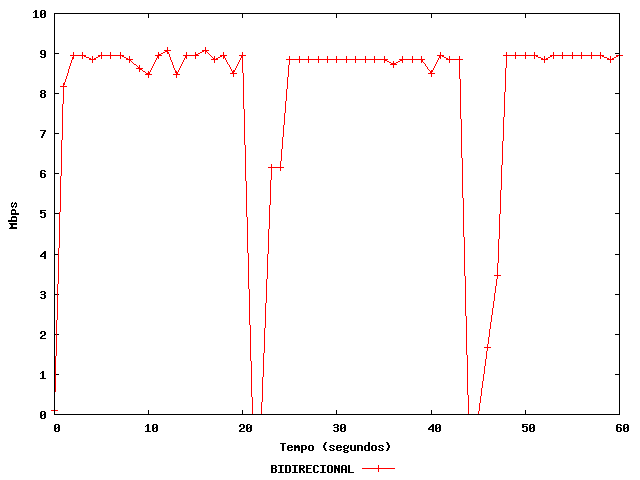
\includegraphics[scale=.6]{figs/banda}
	\caption{Taxa de transmiss�o em \textit{Handover}}
	\label{f_banda}
\end{figure}

A partir dos dados levantados com o teste podemos tirar v�rias conclus�es, entre as quais destacam-se que o \textit{Troughput} suportado pela rede gira em torno de 9 Mbps, este dado esta muito relacionado ao desempenho da m�quina hospedeiro, que cada \textit{handover} � de aproximadamente 3 segundos, h� perdas consider�veis de pacotes que prejudicariam muito comunica��es interativas como videoconfer�ncia e \textit{VoIP}, por�m, navega��o em paginas da \textit{Internet} e visualiza��o de \textit{e-mail} a instabilidade � toler�vel.

Como cen�rio estudo foi simulado todos os tempos medidos s�o estimados. Por�m, segundo algumas bibliografias estudadas que realizaram experimentos fisicamente os tempos medidos na simula��o est�o dentro do esperado.

� percept�vel que as fases que mais comprometem o \textit{handover} do nosso cen�rio s�o as da detec��o de movimento e a configura��o do \textit{care-of-address}. Algumas tentativas podem ser feitas para tentar diminuir a lat�ncia nestas duas fases.

Na tentativa de diminuir o tempo da fase de detec��o de movimento, podemos diminuir o intervalo entre as mensagens de \textit{Router Advertisement} do roteador presente na rede que ir� ser visitada pelo n� m�vel. Pois, � por meio desta mensagem que o n� m�vel detecta o movimento e desencadeia todo o processo de \textit{handover}.

No intuito de verificar se h� uma melhora no processo de handover. O cen�rio estudado foi repetido variando o intervalo entre as mensagens de \textit{Router Advertisement}. O resultado deste teste esta dispon�vel na figura \ref{f_radvd}.

\begin{figure}[!htpb]
	\centering
	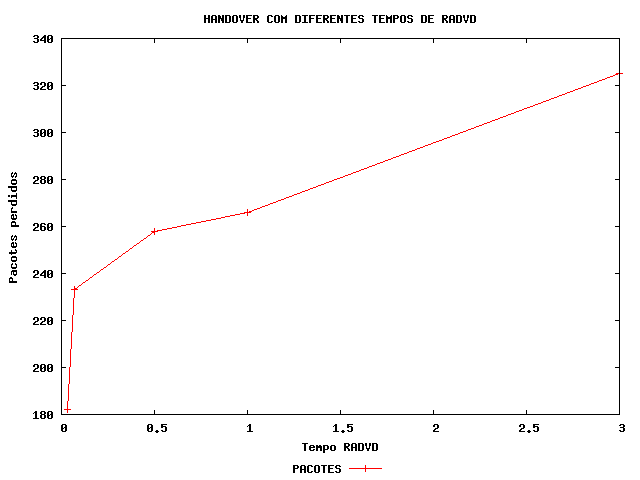
\includegraphics[scale=.6]{figs/radvd}
	\caption{Diferentes intervalos entre as mensagens \textit{Router Advertisement}}
	\label{f_radvd}
\end{figure}

Com os dados levantados, � poss�vel perceber que o intervalo entre as mensagens de \textit{Router Advertisement} esta diretamente ligado com a perda de pacotes durante o \textit{handover}. Por�m, esta n�o � uma boa pr�tica para tentar amenizar a lat�ncia do handover, pois um numero muito grande de mensagens \textit{multicasting} inundaria a rede prejudicando a perfomance principalmente em redes sem fio.

No processo de forma��o de um novo \textit{care-of-address} o DAD � necess�rio para se certificar que o endere�o formado � exclusivo. Para o teste ser bem sucedido nenhum n� vizinho deve enviar um \textit{Neighbor Advertisement}, em resposta ao teste, ou \textit{Neighbor Solicitation}, como o mesmo endere�o em quest�o, em um per�odo de \textit{1000ms} segundo a RFC 2462 \cite{rfc2462}. Este tempo de espera compromete a fase de configura��o do \textit{care-of-address}.

Existe uma vari�vel chamada \textit{dad\_transmits} no kernel do Linux que � usada para configurar o DAD em um n�. Com a inten��o de diminuir a lat�ncia na fase de configura��o do \textit{care-of-address}, n�s configuramos a vari�vel com o valor 0, isso significa que o procedimento de DAD � cancelado, e repetimos o cen�rio estudado.

\section{Resultados}
Com a realiza��o dos experimentos podemos constatar o funcionamento do protocolo e perceber continua��o da comunica��o entre os pontos comunicantes ap�s a mobilidade de forma transparente as camadas superiores a de rede, observar todas as mensagens trocadas no processo e estimar o tempo de lat�ncia com a mobilidade.
O primeiro resultado que se pode obter com a realiza��o do Cen�rio 1, foi o perfeito funcionamento do MIPv6, ocorreram algumas perdas de pacotes, mas o n� m�vel conseguiu continuar sendo alcan�ado pelo seu endere�o domiciliar mesmo n�o estando em sua rede domiciliar.

\section{Cen�rio 2}
\label{s_cenario2}


\begin{figure}[!htpb]
	\centering
	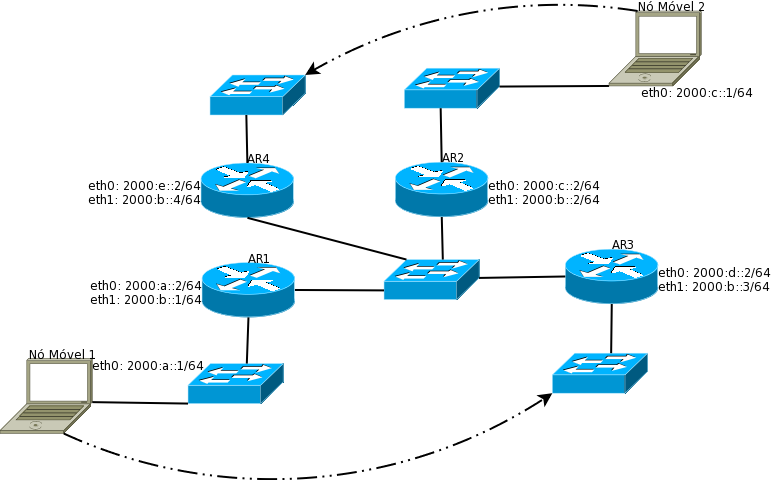
\includegraphics[scale=.37]{figs/cenario2}
	\caption{Topologia do Cen�rio 2}
 	\label{f_cenario2}
\end{figure}

% ----------------------------------------------------------------------- %
% Arquivo: mipl.tex
% ----------------------------------------------------------------------- %
\chapter{Implementa��o do HMIPv6 baseando-se no projeto MIPL}

\section{Implementa��es existentes para Linux dos protocolos de Mobilidade}

O projeto \textit{Mobile IPv6 for Linux} (MIPL) \cite{CitarMIPL} � uma
implementa��o de suporte a mobilidade no IPv6 (RFC 3775), desenvolvida na
Universidade Tecn�logica de Helsinki . O codigo foi desenvolvido acompanhando os
\textit{drafts} da RFC e as vers�es do \textit{kernel linux}. No in�cio do
desenvolvimento, a vers�o do kernel utilizada foi a 2.3.59 e o \textit{draft} 8,
por�m, devido as subst�nciais mudan�as na especifica��o do MIPv6, os gestores 
do projeto decidiram dividir o c�digo fonte uma parte em espa�o de kernel
e outra em espa�o de usu�rio. A �ltima vers�o foi o MIPL 1.1 que trabalhava com
a vers�o 2.4.26 do \textit{kernel linux}.

Mais adiante, iniciou-se o desenvolvimento do MIPL2 pela Universidade de Helsink
juntamente com o projeto USAGI \cite{CitarUsagi}. Nesta nova vers�o houveram
mudan�as significativas: o c�digo foi praticamente todo reescrito e muitas
funcionalidades foram adicionadas em espa�o de usu�rio. Um \textit{daemon}
passou a controlar a sinaliza��o e a detec��o de movimento. A tarefa do
\textit{kernel} passou a ser apenas uma camada de suporte ao MIPv6.

O MIPL2 passou a suportar as �ltimas especifica��es do MIPv6 e passou a utilizar
\textit{framework} XFRM para o suporte a IPSec. � interessante observar tamb�m
que, a partir das �ltimas vers�es do kernel do linux, o suporte ao MIPv6 j� faz
parte da linha principal de desenvolvimento, n�o sendo mais necess�rio aplicar
\textit{patchs}.

No que se refere ao HMIPv6, uma implementa��o foi proposta pela Universidade
de Monash, baseando-se no MIPL 0.94 e na vers�o 2.4 do \textit{kernel linux}.
Tamb�m foram realizadas altera��es no RADVD 0.7.2 para este divulgar mensagens
de MAP. Neste momento, o projeto est� parado e n�o atende mais as necessidades
deste trabalho, pois, ocorreram mudan�as significativas no desenvolvimento do
MIPL. Atualmente a grande maioria dos sistemas j� utilizam a s�rie 2.6 do
\textit{kernel}, ent�o pode-se concluir que n�o h� nenhuma implementa��o
aberta e recente do HMIPv6.

O trabalho prop�e-se, ent�o desenvolver uma  implementa��o experimental
atualizada do HMIPv6, baseando-se na �ltima vers�o est�vel do projeto MIPL
e utilizando a vers�o 0.7.2 do RADVD alterado pelo projeto da Universidade de
Monash.

\section{Estudo do c�digo do projeto MIPL}
Com fins de gerar uma vers�o do HMIPv6 a partir do projeto MIP, iniciou-se
um estudo aprofundado do c�digo fonte do MIPL. O estudo do c�digo do
MIPL2 foi realizado na sua �ltima vers�o est�vel, anunciada pelo projeto USAGI
como umip-0.4. O MIPL � um projeto de codigo aberto sobre a licen�a GPL vers�o
2, escrito na linguagem de programa��o C.

O programa � executado na forma de um \textit{daemon} chamado de \textit{mip6d},
ou seja, um processo executado no segundo plano e que n�o est� associado a um
terminal controlador \ref{stevens}. Este mesmo \textit{daemon} desempenha o
papel de n� m�vel, de agente domiciliar e de n� correspondente. A sua fun��o �
definida em um arquivo de configura��o, sendo que todos os n�s s�o em pontencial
um n� correspondente.

O foco principal do estudo foi na parte respons�vel pelo
funcionamento do n� m�vel, pois as principais mudan�as do MIPv6 para o HMIPv6 �
a funcionalidade deste n�. O agente MAP possui, basicamente, o mesmo
comportamento de um agente domiciliar, a n�o ser pelo de fato de possuir uma
rede com prefixo a partir do qual ser�o criados RCoAs. Al�m do que, todo o
projeto � de alta complexidade, envolvendo o uso de v�rias bibliotecas, o que
demandaria um tempo grande de estudo. � bom lembrar tamb�m que, com fins de
delimitar o escopo do trabalho, foram desconsiderados todos os mecanismos de
seguran�a do HMIPv6.

\subsection{Intera��o entre o \textit{kernel} e o MIPL}
Geralmente tudo o que fizemos, enquanto trabalhamos em um sistema Linux, est�
sendo executado em em espa�o de usu�rio, por exemplo: um editor de texto, um
navegador, servidor X. Em contraste com isso, o \textit{kernel} executa as suas
tarefas em espa�o de \textit{kernel}, com acesso � instru��es privilegiadas,
total controle da mem�ria e do sistema de interrup��es. O principal motivo para
esta separa��o entre dados dos processos do usu�rio e do
\textit{kernel}, � evitar que um perturbe o outro, o que resultaria numa
diminui��o do desempenho, problemas de seguran�a e instabilidades do sistema
\ref{spaces}.

Os motivos levantados acima foram os que levaram os desenvolvedores a passarem a
maioria da implementa��o do protocolo MIPv6 para espa�o de usu�rio, o que torna
desenvolvimento mais f�cil, seguro e independente de vers�o de \textit{kernel}.
Por�m o MIPL precisa de uma interface para a troca de informa��es entre o
\textit{kernel} e espa�o de usu�rio. A troca de informa��o do entre
\textit{kernel} e o espa�o de usu�rio � realizada atrav�s do
\textit{netlink}. O \textit{netlink} consiste em uma extens�o da interface de
soquetes padr�o, que proporciona uma comunica��o bidirecional entre
\textit{kernel} e o espa�o de usu�rio. O soquete \textit{netlink} usa endere�os
da fam�lia AF\_NETLINK, comparado ao AF\_INET usado pelos soquetes TCP/IP
\ref{netlink}.

O soquete \textit{netlink} � a forma utilizada pelo MIPL para:
\begin{itemize}
 \item acessar as informa��es do MIPv6 no \textit{kernel};
 \item alterar endere�os IP's;
 \item manipular tabelas de roteamento e regras das pol�ticas de uso destas
tabelas;
 \item criar t�neis.
\end{itemize}

Os soquetes brutos tamb�m s�o utilizados pelo MIPL para permitir a leitura e
envio de pacotes puramente IP sem a interfer�ncia do \textit{kernel}\ref{raw}.
Em condi��es normais quando o kernel n�o entende o campo de protocolo do
datagrama IP, como por exemplo, os que possuim cabe�alho de mobilidade, eles s�o
passados diretamente para um soquete bruto. O �nico processamento feito pelo
\textit{kernel} � a verifica��o m�nima de alguns campos de cabe�alho IP.

Esta capacidade permite que tais pacotes possam ser tratados por aplica��es
independentes de inser��o de c�digos especiais em \textit{kernel}, neste caso o
\textit{daemon} MIPL.

\subsection{\textit{Threads} importantes do MIPL}
No seu funcionamento, o \textit{daemon} do MIPL necessita realizar v�rias
tarefas, por exemplo, interagir com o \textit{kernel}. Para realizar as v�rias
fun��es que permitem o funcionamento do protocolo MIPv6, o programa utiliza a
t�cnica de \textit{Multithreading}. A seguir s�o listadas \textit{threads} que
executam no \textit{daemon} e a figura \ref{f_mipl_kernel_blocks} mostra a forma
que algumas delas se relacionam com o \textit{kernel}.

\subsubsection{\textit{runner}}
Durante a sua execu��o, o \textit{mip6d} necessita agendar tarefas para serem
executadas. Por exemplo, caso o tempo de vida de um endere�o expirar ele precisa
ser removido, para isso, o \textit{daemon} cria uma tarefa que remove o
endere�o da interface, e a insere em uma fila global de tarefas.

Para inserir tarefas na fila o \textit{daemon} utiliza a fun��o
\textit{add\_task\_abs}, passando como par�metro:
\begin{itemize}
 \item o tempo em milisegundos para a execu��o da tarefa;
 \item ponteiro para fun��o que deve ser chamada quando o tempo da tarefa
expirar.
\end{itemize}

\begin{figure}[!htpb]
	\centering
	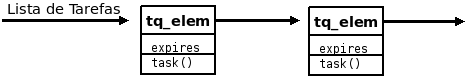
\includegraphics[scale=.8]{figs/task}
	\caption{Fila de tarefas agendadas do MIPL}
	\label{f_mipl_tasks}
\end{figure}

A \textit{thread runner}, fica percorrendo a fila de tarefas(ver figura
\ref{f_mipl_tasks}) e quando o tempo da tarefa expira, executa uma fun��o
associada, previamente registrada.

\subsubsection{\textit{icmp6\_listen}}
O MIPL cria uma \textit{thread} para escutar mensagens ICMPv6 e para isso cria
um soquete bruto. Por�m, h� muitas mensagens ICMPv6, por isso, para reduzir o
n�mero de pacotes passados do \textit{kernel} para a aplica��o, � fornecido um
filtro especifico pela aplica��o. Na tabela \ref{t_mipl_icmp} � poss�vel
observar as mensagens ICMPv6 que ser�o tratadas pelo MIPL.

\begin{table}[!htpb]
\centering
\begin{small}
  \setlength{\tabcolsep}{3pt}
\begin{tabular}{|c|c|c|c|}\hline
\raisebox{1.5ex}{Fun��o mip6d} & \raisebox{1.5ex}{Mensagem Filtrada} &
\raisebox{1.5ex}{Fun��o}\\ \hline
N� M�vel & ND\_ROUTER\_ADVERT & An�ncio de roteadores  \\ 
	 & ND\_NEIGHBOR\_ADVERT & An�ncio de vizinhan�a \\ 
	 & MIP\_HA\_DISCOVERY\_REPLY & Resposta de descoberta de agente
domiciliar \\
	 & ICMP6\_PARAM\_PROB & askdfj;al \\
	 & ICMP6\_DST\_UNREACH & Destino inalcan��vel \\ \hline
Agente Domiciliar & MIP\_PREFIX\_SOLICIT & Solicita��o de prefixo \\
		  & MIP\_HA\_DISCOVERY\_REQUEST & Descoberta de agente
domiciliar \\
		  & ND\_ROUTER\_ADVERT & An�ncio de roteadores \\
		  & ICMP6\_DST\_UNREACH & Destino inalcan��vel; \\ \hline
\end{tabular} 
\end{small}
\caption{Filtros para os pacotes ICMPv6 feitos pelo MIPL}
\label{t_mipl_icmp}
\end{table} 

Durante a execu��o do \textit{daemon} � feita a instala��o de manipuladores, que
tratam as mensagens, em uma lista global. Ao receber uma das mensagens ICMPv6
filtradas, a \textit{thread} percorre a lista de manipuladores e chama a fun��o
para tratar a mensagem.

\begin{figure}[!htpb]
	\centering
	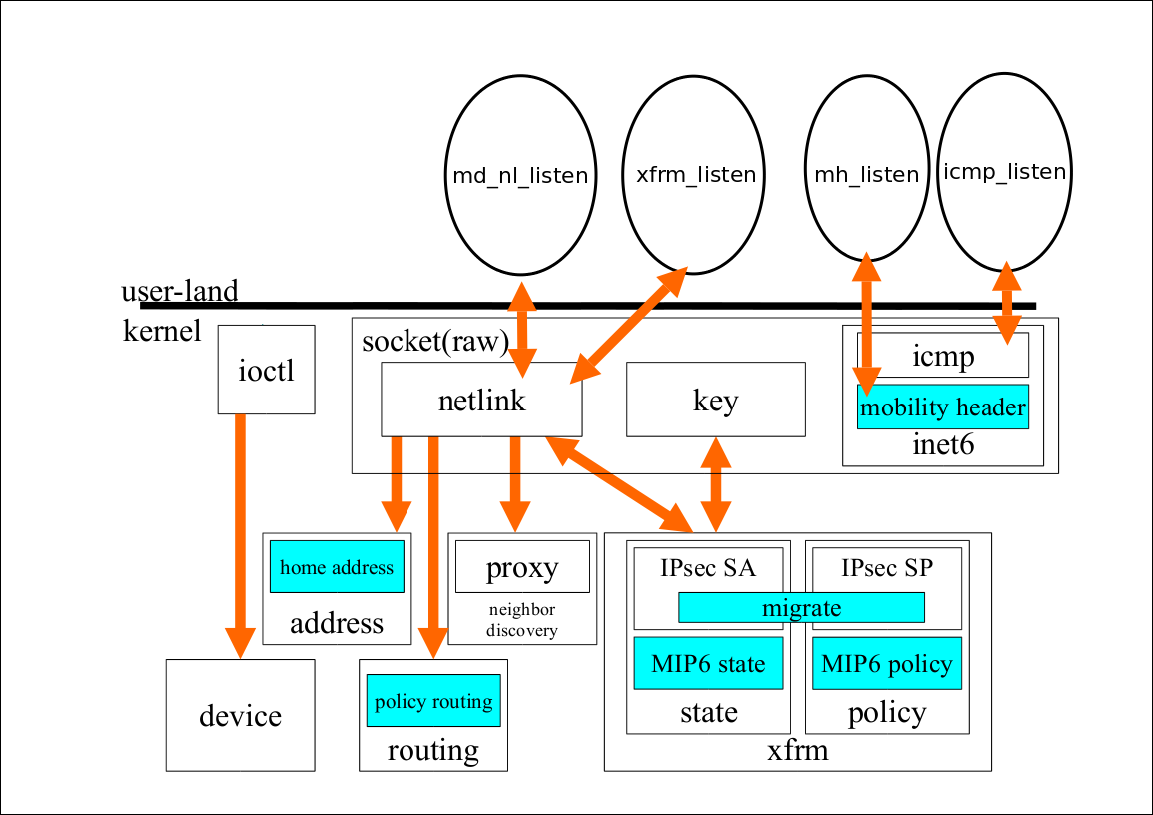
\includegraphics[scale=.27]{figs/mipl_kernel_block}
	\caption{Interfaces utilizadas pelo MIPL para fazer a comunica��o com o
kernel\cite{CitarFigura}}
	\label{f_mipl_kernel_blocks}
\end{figure}

\subsubsection{\textit{mh\_listen}}
\textit{Thread} criada para escutar a chegada de pacotes IPv6 com cabe�alho de
mobilidade. O seu funcionamento � semelhante a \textit{thread icmp6\_listen}: ao
receber uma mensagem com o cabe�alho de mobilidade chama um manipulador,
previamente instalado em uma lista global, para tratar a mensagem.

\subsubsection{\textit{xfrm\_listen}}
O \textit{daemon} cria a \textit{thread xfrm\_listen} que escuta mensagens
\textit{netlink} do \textit{framework} XFRM. Um manipulador � instalado para
tratar essas mensagens. As mensagens s�o: XFRM\_MSG\_ACQUIRE e
XFRM\_MSG\_REPORT.

\subsubsection{\textit{md\_nl\_listen}}
O \textit{mip6d} cria uma \textit{thread} para tratar mensagens \textit{netlink}
do tipo NETLINK\_ROUTE enviadas pelo \textit{kernel}. Esta \textit{thread} �
executada somente no n� m�vel.

A \textit{thread} ao receber uma mensagem \textit{netlink}, chama o manipulador
instalado para trat�-la. As mensagens tratadas pelo manipulador s�o as que
informam:
\begin{itemize}
 \item a interface ou liga��o: ligado ou desligado;
 \item as mudan�as no estado da alcan�abilidade do roteador padr�o;
 \item os \textit{Care-of-address} novos ou removidos.
\end{itemize}

\subsubsection{\textit{vt\_server\_recv}}
� possivel habilitar em tempo de compila��o um terminal virtual. O terminal
virtual permite que os usu�rios se conectem ao \textit{daemon}, via protocolo
\textit{telnet}, para obter informa��es sobre o MIPv6, por exemplo:
\begin{itemize}
 \item O tempo de vida do prefixo do agente domiciliar;
 \item O estado do \textit{Binding cache};
 \item A Lista de \textit{Bindig Updates}.
\end{itemize}

A \textit{thread} \textit{vt\_server\_recv} � criada para responder as conex�es
para o terminal virtual, que � executado na porta 7777.

\subsubsection{\textit{sigh}}
O \textit{mip6d} implementa uma \textit{thread} que � respons�vel por fazer o
tratamento de alguns sinais do sistema. Os sinais que passam a ser tratados pela
aplica��o s�o:
\begin{description}
 \item[SIGHUP:] Significa o reinicio do programa, o \textit{daemon} ao receber
esse sinal executa a fun��o \textit{reinit};
\item[SIGINT:] Causa a interrup��o do programa, em termos pr�ticos � o sinal
recebido quando se pressiona as teclas \textit{Control+C}. Neste caso ao receber
este sinal o \textit{daemon} chama a fun��o \textit{terminate};
\item[SIGTERM:] Solicita��o de t�rmino do programa, neste caso o \textit{daemon}
tamb�m chama a fun��o \textit{terminate}.
 \end{description}

� de extrema import�ncia o tratamento destes sinais pelo \textit{daemon}, pois
ao finalizar o programa � preciso deletar eventuais endere�os IP's, t�neis,
tabelas de roteamento.

\subsection{Detec��o de Movimento}
O algoritmo de detec��o de movimento do MIPL � inteiramente baseado na escuta
das mensagens de an�ncio de roteadores. O n� m�vel est� constantemente escutando
as mensagens de RA, sendo que o n� percebe o movimento quando:
\begin{itemize}
 \item o seu roteador padr�o torne-se inalcan��vel; para tanto, o n� m�vel de
tempos em tempos, verifica o roteador com um \textit{Neighbor Solicitation};
 \item passa a receber mensagens de outro roteador e para de escutar
mensagens do anterior.
\end{itemize}

Embora o MIPL seja uma extens�o da pilha IPv6 padr�o do \textit{Linux},
apresenta algumas caracter�sticas sobre administra��o de roteadores:
\begin{enumerate}
 \item O MIPL possui a sua pr�pria lista de roteadores. Esta lista cont�m o 
atual roteador de acesso, bem como roteadores que n�o s�o atualmente
utilizados, mas com tempo de vida n�o expirados;
 \item o MIPL for�a atualiza��es na tabela de roteamento ap�s receber um an�ncio
de novo roteador, e apaga todas as informa��es de roteamento que n�o s�o do
prefixo atual.
\end{enumerate}
Devido a estas duas caracter�sticas, o MIPL sempe escolhe um novo roteador. Este
m�todo de sele��o agressiva de roteadores traz uma melhora na detec��o de 
movimento, ou seja, no tempo de \textit{handover}.

\section{Altera��es no MIPL para obter o HMIPv6}
A primeira implementa��o necess�ria foi dar suporte ao MIPL a leitura das
mensagens RA divulgadas pelos MAP's, pois s�o elas que permitem a cria��o do
endere�o RCoA. No manipulador de mensagens RA foi adicionado o suporte para
a leitura da op��o de MAP na mensagem RA. Foi criada uma estrutura de dados
para o MAP e fun��es para manipula��o desta estrutura. Na estrutura de dados do
roteador foi adicionado uma lista de MAP's. A estrutura � mostrada a seguir.

\begin{lstlisting}
struct map_list_entry
{
    struct list_head list;
    struct timespec timestamp;
    struct tq_elem tqe;
    struct nd_opt_map map;
    struct in6_addr rcoa;
    int used;
};
\end{lstlisting}
A estrutura cont�m:
\begin{itemize}
 \item os campos da op��o de MAP da mensagem RA;
 \item tempo de vida do roteador que entregou a mensagem;
 \item endere�o RCoA criado a partir do endere�o do MAP;
 \item estrutura de dados que permite criar tarefas para serem agendadas;
\end{itemize}

No processamento da mensagem RA foram adicionados novos eventos de
movimento:\textbf{ME\_MAP\_NEW}, \textbf{ME\_MAP\_UPDATE} e
\textbf{ME\_MAP\_EXPIRED} Estes eventos tem a fun��o de colher os
dados que ser�o utilizados no momento do registro e  manter os dados para o
funcionamento do protocolo.

Foi criada tamb�m uma estrutura de dados para o RCoA tendo sido adicionada na
estrutura do agente domiciliar. As informa��es contidas na estrutura ser�o
utilizadas no momento da forma��o das mensagens de BU e no controle do registro.

\begin{lstlisting}
struct rcoa_addr_info {
    struct mn_addr rcoa; /* Home address for MAP */
    uint8_t mlen;
    uint8_t map_reg_status;
    struct in6_addr map_prefix;
    struct in6_addr map_addr;
    int pend_ba;
    int site;
    int if_tunnel;
};
\end{lstlisting}

Outas implementa��es foram realizadas no n� m�vel, quais sejam:
\begin {itemize}
 \item  foi acrescentado ao mecanismo de registro, um suporte ao envio do BU
para o MAP;
\item altera��o da mensagem de BU para o agente domiciliar;
\item cria��o do t�nel, com o MAP;
\item e modifica��o do t�nel com o agente domiciliar.
\end {itemize}

Algo interessante de salientar � que toda a parte de tomada de decis�o sobre o
movimento se manteve e as altera��es atuam somente na forma do registro com
os agentes.

\subsection{Detalhes do funcionamento}
A seguir, uma descri��o das implementa��es efetuadas no MIPL em um movimento
para um novo dom�nio:
\begin{enumerate}
 \item Ao receber uma mensagem RA de um novo roteador de acesso:
\begin{itemize}
 \item as op��es de MAP s�o lidas;
 \item uma lista de MAP's � criada na estrutura do roteador.
\end{itemize}
 \item Um novo MAP dispara um evento de movimento do tipo \textbf{ME\_MAP\_NEW}
que:
\begin{itemize}
 \item faz escolha de um MAP na lista de roteadores, baseado na dist�ncia em
saltos do MAP;
 \item cria um t�nel para o MAP;
 \item adiciona o RCoA na interface do t�nel;
 \item define o RCoA na estrutura do agente domiciliar, utilizado no envio do
BU.
\end{itemize}
 \item o movimento � detectado, usando o c�digo normal do MIPL. O registro
deve ser, ent�o, realizado com os agentes:
\begin{itemize}
 \item enviado BU para o MAP com os campos:
\begin{itemize}
 \item Origem = RCoA
 \item Destino = endere�o MAP
 \item Care-of-Adress = LCoA
\end{itemize}
 \item enviado BU para agente domiciliar com os campos:
 \begin{itemize}
  \item Origem = endere�o domiciliar
  \item Destino = endere�o agente domiciliar
  \item Care-of-Adress = RCoA
 \end{itemize}
\end{itemize}
 \item Ap�s o envio dos BU's, os t�neis devem ser modificados:
 \begin{itemize}
  \item T�nel entre n� m�vel e MAP: o ponto final � a interface de rede.
  \item T�nel entre n� m�vel e agente domiciliar: o ponto final � o t�nel entre
n� m�vel e MAP.
 \end{itemize}
 \item Periodicamente, com a chegada dos RA's, o evento de movimento
\textbf{ME\_MAP\_UDATE} � disparado e o tempo de vida do RCoA � atualizado.
\end{enumerate}

\subsection{Problemas conhecidos}
Considerando o car�ter experimental do trabalho, a disponibilidade de tempo
para a sua execu��o e a alta
complexidade do c�digo do MIPL, pode-se dizer que muito trabalho deve ainda ser
realizado para a obten��o de uma vers�o completa do HMIPv6. No que se refere a
implementa��o efetuada, alguns problemas podem, em particular, ser apontados:
\begin{itemize}
 \item aus�ncia de suporte a otimiza��o de rotas;
 \item aus�ncia de suporte a seguran�a (IPSec);
 \item aus�ncia de suporte ao HMIPv6 em arquivo de configura��o, somente em
tempo de compila��o;
 \item sem tarefas para deletar MAP's expirados;
 \item problema ao receber BA provindo do MAP, o que ocasiona problemas em
mobilidade em um mesmo dom�nio;
 \item problemas no retorno para rede domiciliar.
\end{itemize}

% ----------------------------------------------------------------------- %
% Arquivo: hmipv6.tex
% ----------------------------------------------------------------------- %
\chapter{Vis�o geral do protocolo HMIPv6}
\label{c_hmipv6}
O modelo do protocolo MIPv6 apresenta alguns problemas que comprometem a sua escalabilidade na \textit{Internet}, alguns desses puderam ser observados nos cen�rios estudados. Dentre estes problemas podemos destacar:
\begin{itemize}
 \item tempo na detec��o do movimento;
 \item tempo na configura��o do novo endere�o na rede visitada, o \textit{care-of-address};
 \item tempo do registro com o seu agente domiciliar;
\end{itemize}

Em um ambiente utilizando o MIPv6 com um excessivo numero de n�s m�veis a tend�ncia � a perda na qualidade de servi�o e o aumento do \textit{delay} na entrega dos pacotes.

Com o intuito de minimizar os efeitos dos longos retardos no envio dos \textit{Binding Updates}, para o registro com o agente domiciliar ou o n� correspondente, e reduzir o tr�fego de pacotes de controle na \textit{Internet} foi proposto um protocolo complementar ao MIPv6 o IPv6 M�vel Hier�rquico (HMIPv6).

%ref
A id�ia principal do protocolo � tratar a mobilidade global e local de formas distintas, uma movimenta��o local pode ser entendida como uma que acontece em um mesmo \textit{site} e a global entre \textit{sites}. Podemos definir um  \textit{site} como uma dimens�o arbitr�ria, e pode ser, por exemplo, uma rede de uma empresa ou universidade com uma ou mais sub-redes.

%ref
Um estudo sobre os padr�es de mobilidade analisou diversos profissionais, mostrou que 69\% das movimenta��es s�o locais independente deles possu�rem algum dispositivo m�vel. Este dado mostra que o modelo hier�rquico � mais adequado para o uso na \textit{Internet}. As principais vantagens seriam a diminui��o no tempo do \textit{handover} e do tr�fego enviado para � \textit{Internet} com sinaliza��o.

\section{Terminologia do HMIPv6}
\begin{description}
 \item[Roteador de acesso (RA):] � o roteador padr�o do n� m�vel, recebe os dados de sa�da do n� m�vel.
 \item[\textit{Mobility Anchor Point} (MAP):] � um roteador localizado na rede visitada, o MAP � usado como um agente domiciliar pelo n� m�vel. Um ou mais MAPs podem existir em uma rede visitada.
 \item[N� m�vel HMIPv6:] � um n� m�vel capaz de receber e processar mensagens do roteador padr�o que contenham a op��o MAP. Um n� m�vel HMIPv6 deve ser apto para enviar \textit{Binding Updates} locais com o bit M ligado.
 \item[Regional \textit{care-of-address} (RCoA):] � o endere�o obtido pelo n� m�vel na rede visitado com o mesmo prefixo de rede do MAP. Ele � auto-configurado quando recebe a op��o de MAP divulgada nas mensagens do roteador padr�o.
 \item[\textit{Link care-of-address} (LCoA):] � o endere�o configurado pelo n� m�vel com o mesmo prefixo do roteador padr�o. Uma simples refer�ncia ao care-of-address.
 \item[\textit{Binding Update} local:] � o \textit{Binding Update} que o n� m�vel envia para o MAP fazer a associa��o do LCoA com o RCoA.
 \end{description}

\section{Funcionamento}
A principal mudan�a no HMIPv6 em rela��o ao MIPv6 foi � indtrodu��o de um novo agente, o MAP que nada mais � do que um roteador utilizado para gerenciar a mobilidade. O funcionamento do agente domiciliar e do n� corresponde permanece id�ntico ao do MIPv6. Assim como no MIPv6 o funcionamento do HMIPv6 idepende da tecnologia de acesso.

Assim que um n� movel entra em um \textit{site} com a presen�a de um MAP, ele se conecta com um RA e auto-configura dois endere�os o RCoA baseado no mesmo prefixo de rede do MAP e outro o LCoA com o mesmo prefixo do RA. Ent�o o n� m�vel envia um \textit{Binding Update} para o MAP para que este fa�a a associa��o do RCoA com o LCoA. Outros \textit{Binding Updates} tamb�m s�o enviados para o agente domiciliar e os n�s correspondentes, neste caso para que estes fa�am a associa��o do endere�o domiciliar com o RCoA. Se o n� m�vel estiver se comunicando com correspondes locais, ou seja, do mesmo \textit{site} ele deve enviar um \textit{Binding Update} para � associa��o do endere�o domiciliar com o LCoA.

O funcionamento do MAP � semelhante ao do agente domiciliar, ele intercepta os pacotes originados do agente domiciliar e dos n�s correspondentes destinados ao RCoA e ent�o os envia via t�nel ao LCoA. Um t�nel bidirecional � estabelecido entre o MAP e o n� m�vel, que � usado para enviar todos os pacotes oriundos do n� m�vel, exceto os com destino aos correspondentes locais.

As principais formas de atua��o propostas pelo protocolo s�o quando o n� m�vel se desloca dentro de um mesmo \textit{site} (mobilidade local) e entre \textit{sites} (mobilidade global):
\begin{description}
 \item[Mobilidade local:] quando o n� m�vel troca somente o seu LCoA, � necess�rio o envio de \textit{Binding Updates} para o MAP e os correspondentes locais. Como resultado os pacotes com origem do agente domiciliar e dos n�s correspondentes ainda s�o enviandos para o mesmo RCoA, assim minimizando o tempo do \textit{handover} e a perda de pacotes, tamb�m notamos que todo tr�fego gerado � dentro do mesmo \textit{site}.
\begin{figure}[!htpb]
	\centering
	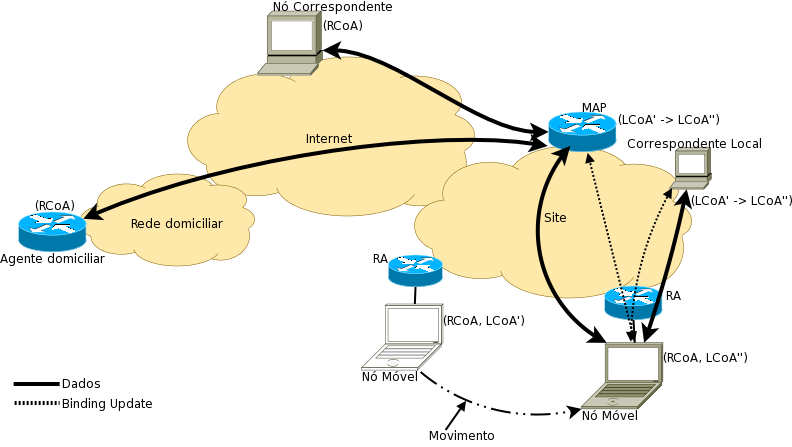
\includegraphics[scale=.45]{figs/intra_site}
 	\label{f_intra}
	\caption{Mobilidade Local}
\end{figure}

\item[Mobilidade global:] neste caso o n� m�vel reconfigura o seu RCoA e LCoA, e envia Binding Updates para o MAP, os n�s comunicantes fora do \textit{site} informando o novo RCoA e os n�s do mesmo site para informar o LCoA.
\begin{figure}[!htpb]
	\centering
	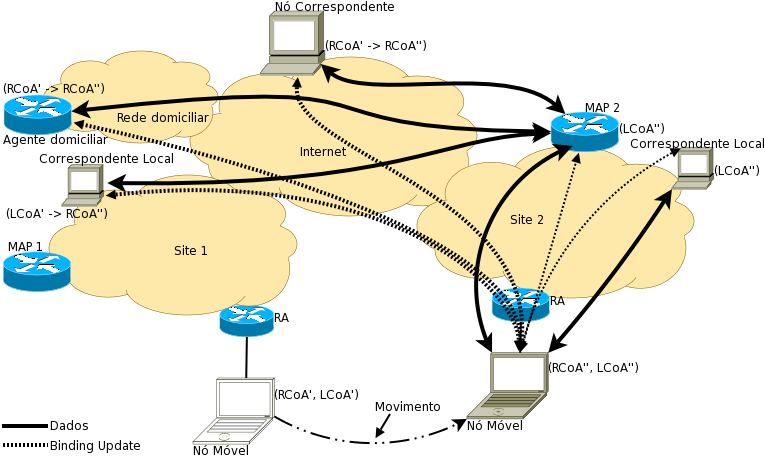
\includegraphics[scale=.45]{figs/inter_site}
 	\label{f_inter}
	\caption{Mobilidade Global}
\end{figure}
\end{description}

Podemos perceber que em algumas vezes o n� m�vel deve preferir atuar como no MIPv6 para tornar mais simples o seu funcionamento. Neste caso a rede visitada se encontra pr�xima ao agente domiciliar e n�o se faz necess�rio o uso do MAP, a discuss�o sobre este tipo de cen�rio n�o faz parte do escopo deste documento. 

\section{Envio de \textit{Binding Updates}}
%ref
Ap�s o evento de mobilidade e o n� m�vel auto-configurou o seu RCoA ele precisa enviar um \textit{Binding Update} para o MAP. O pacote desta mensagem deve seguir os seguintes requisitos, definidos em:
\begin{itemize}
 \item bit A (\textit{acknowledge}) deve estar ligado;
 \item bit M (\textit{map registration}) deve estar ligado;
 \item o RCoA na op��o de agente domiciliar;
 \item o LCoA deve ser usado como endere�o de origem do \textit{Binding Update};
\end{itemize}
O \textit{Binding Update} ir� associar o RCoA com o LCoA, similarmente como um endere�o domiciliar. O MAP far� o teste de duplicidade (DAD) do RCoA, somente no primeiro \textit{Binding Update}, e retornar� um \textit{Binding Acknowledgement} para o n� m�vel.

A especifica��o do protocolo permite que um n� m�vel tenha mais de um RCoA se recebeu mais de uma op��o de MAP, para todos os RCoAs devem ser feito um Binding Update. O n� m�vel n�o deve fazer um multi-n�vel hier�rquico, pois ir� diminuir a efici�ncia e a performance do protocolo muitos 

Depois de fazer o registro com o MAP o n� m�vel deve fazer a associa��o do RCoA com o endere�o domiciliar no agente domiciliar e nos n�s correspondentes. A mensagem de \textit{Binding Update} deve ser envianda utilizando a op��o de \textit{care-of-address} alternativo preenchida com o RCoA e o tempo de vida deve ser menor do recebido no \textit{Binding Acknowledgement} do registro com o MAP.

\section{Descoberta de um MAP}
Esta se��o descreve como um n� m�vel obtem o endere�o do MAP e seu prefixo de rede, e como ARs presentes no \textit{site} descobrem os MAPs. Dois m�todos s�o definidos para o descobrimento do MAP:
 
\begin{description}
 \item[Descobrimento din�mico:] � baseado na propaga��o da op��o de MAP nas mensagens de \textit{Router Advertisements}. Na op��o de MAP est�o presentes o endere�o global do MAP, seu prefixo de rede, um vetor de dist�ncia baseado nos saltos da mensagem at� a chegada no n� m�vel, esta op��o influenciar� na escolha do MAP padr�o, e um MAP particular como prefer�ncia. Neste m�todo os ARs devem ser configurados para receberem as mensagens com op��es de MAP e re-enviarem incrementando o vetor de dist�ncia.
 \item[Configura��o manual:] neste m�todo a op��o de MAP � configurada manualmente nos ARs por um administrador da rede, em muitos \textit{sites} esse � o mescanismo padr�o. Tamb�m deve ser poss�vel a configura��o por mecanismos din�micos.
 \end{description}

% ----------------------------------------------------------------------- %
% Arquivo: conclusoes.tex
% ----------------------------------------------------------------------- %

\chapter{Conclus�es}
\label{c_conclusoes}

Este trabalho procurou mostrar como dever� ser a apresenta��o da monografia a ser submetida � Coordena��o do Curso Superior de Tecnologia em Sistemas de Telecomunica��es do Centro Federal de Educa��o Tecnol�gica de Santa Catarina para a obten��o do diploma de Tecn�logo em Sistemas de Telecomunica��es.

No cap�tulo \ref{c_introducao} foi feita uma pequena introdu��o. No cap�tulo  foram apresentados alguns coment�rios sobre figuras. E no cap�tulo  foi apresentada uma forma para inserir tabela.

Como trabalho futuro, fica a reescrita do texto deste documento de forma que ele possam indicar informa��es espec�ficas a formata��o do documento. Como o tamanho da fonte utilizada, o espa�amento da borda, o alinhamento e n�mera��o das se��es e cap�tulos, etc.

% inclus�o de ap�ndices (se houver)
% \apendice
% \include{apendice1}

% inclus�o de anexos (se houver)
\anexo
% ----------------------------------------------------------------------- %
% Arquivo: anexo1.tex
% ----------------------------------------------------------------------- %

\chapter{Gerador de tr�fego}
\label{c_anexo1}

\begin{verbatim}
 /*
* gen-0.1
*
* (c) 2008 Cleiber Marques
*
* This program is free software; you can redistribute it and /or
* modify it under the terms of the GNU General Public License
* as published by the Free Software Foundation; either version
* 2 of the License, or (at your option) any later version.
*
*/

#include <stdio.h>
#include <stdlib.h>
#include <unistd.h>
#include <errno.h>
#include <string.h>
#include <time.h>
#include <sys/types.h>
#include <sys/socket.h>
#include <netinet/in.h>
#include <arpa/inet.h>
#include <netdb.h>

#define PORT 4950
#define SIZE_PACK 100
#define IPV6 
/*#define LOOP*/

int main(int argc, char **argv)
{
  int fd, numbytes, len;
  char buf[SIZE_PACK];
#ifdef IPV6
  struct sockaddr_in6 gen, rcv;
#else
  struct sockaddr_in gen, rcv;
#endif
  struct tm *local;
  time_t t;
  char addr[INET6_ADDRSTRLEN];
  /* Cria um socket UDP */
#ifdef IPV6
  printf("Program version IPv6\n");
  if (!(fd = socket(AF_INET6, SOCK_DGRAM, 0))) {
#else
  printf("Program version IPv4\n");
  if (!(fd = socket(AF_INET, SOCK_DGRAM, 0))) {
#endif
    fprintf(stderr, "Error in create socket\n");
    exit (1);
  }
  bzero(&gen, sizeof(gen));
#ifdef IPV6
  gen.sin6_family = AF_INET6;
  gen.sin6_port = htons(PORT);
#else
  gen.sin_family = AF_INET;
  gen.sin_port = htons(PORT);
#endif
  if(argc == 1) {
#ifdef IPV6
    gen.sin6_addr = in6addr_any;
#else
    gen.sin_addr.s_addr = INADDR_ANY;
#endif
    /* Bind */
    if (bind(fd, (struct sockaddr *)&gen, sizeof(gen)) == -1) {
      fprintf(stderr, "Error in bind\n");
      exit(1);
    }
    while(1) {
      len = sizeof(rcv);
      /* Recebe pacote */
      if ((numbytes=recvfrom(fd, buf, SIZE_PACK , 0,
          (struct sockaddr *)&rcv, &len)) == -1) {
        fprintf(stderr,"Error in recvfrom\n");
        exit(1);
      }
      /* Pega a hora do sistema e imprime */
      t = time(NULL);
      local = localtime(&t);
#ifdef LOOP
      /* Envia pacote */
      if ((numbytes = sendto(fd, buf, SIZE_PACK, 0,
          (struct sockaddr *)&rcv, sizeof(gen))) == -1) 
        fprintf(stderr, "Error in sendto\n");
#endif
      /* Imprime log */
#ifdef IPV6
      inet_ntop(AF_INET6, &rcv.sin6_addr, addr, sizeof(addr));
      printf("Receive packet [%d:%d:%d] %d bytes from %s seq=%d\n", local->tm_hour,
        local->tm_min, local->tm_sec, numbytes, addr, buf[0]);
#else
      printf("Receive packet [%d:%d:%d] %d bytes from %s seq=%d\n", local->tm_hour,
        local->tm_min, local->tm_sec, numbytes, inet_ntoa(rcv.sin_addr), buf[0]);
#endif
    }
  } else {
    int count = 0, i;
#ifdef IPV6
    inet_pton(AF_INET6, argv[1], &gen.sin6_addr);
#else
    inet_pton(AF_INET, argv[1], &gen.sin_addr);
#endif
    while(1) {
      srand(time(NULL));

      /* Completa o pacote com numeros randomicos */
      for(i=0; i<SIZE_PACK; i++)
        buf[i] = rand() % 10; 
      /* Envia pacote */
      if ((numbytes = sendto(fd, buf, SIZE_PACK, 0,
          (struct sockaddr *)&gen, sizeof(gen))) == -1) {
        fprintf(stderr, "Error in sendto\n");
        exit(1);
      }
      /* Pega a hora do sistema e imprime  */
      t = time(NULL);
      local = localtime(&t);
#ifdef LOOP
      len = sizeof(rcv);
      /* Recebe pacote */
      if ((numbytes=recvfrom(fd, buf, SIZE_PACK , 0,
          (struct sockaddr *)&rcv, &len)) == -1) {
        fprintf(stderr,"Error in recvfrom\n");
        exit(1);
      }
#endif
      /* Imprime log */
      printf("Send packet [%d:%d:%d] %d bytes from %s seq=%d\n",
        local->tm_hour, local->tm_min, local->tm_sec, numbytes, argv[1], buf[0]);
      sleep(1);
    }
  }
}
\end{verbatim}

% ----------------------------------------------------------------------- %
% Arquivo: anexo2.tex
% ----------------------------------------------------------------------- %

\chapter{Cen�rios}
\label{c_anexo2}

\begin{verbatim}
#!/bin/sh
#
# cenario.sh:	script que gera as m�quinas e switches virtuais para os
#               dois cen�rios definidos no trabalho.
# Uso: 		./cenario.sh <cenario> <modo>
# cenario:	numero do cen�rio, 1 ou 2;
# modo:		modo de opera��o, 1 para tunelamento bidirecional,
#		2 para otimiza��o de rotas.
# 
WD=~/vm
FSYS=DebianFS
LINUX=$WD/linux
CENARIO=$1
$MODO=$2
echo "Iniciando Cenario $CENARIO"
echo "Limpando cows"
rm $WD/cow-*
echo "Limpando pipes"
rm /tmp/net*
echo $MODO > $WD/conf
echo "Lancamento dos switches"
xterm -geometry 80x5 -T NET100 -e "uml_switch_mob -mob -unix /tmp/net100.ctl" &
if [ $CENARIO -eq 1 ]
then
  xterm -geometry 80x5 -T NET200 -e "uml_switch  -unix /tmp/net200.ctl"  &
else
  xterm -geometry 80x5 -T NET200 -e "uml_switch_mob -mob -unix /tmp/net200.ctl" &
fi
  xterm -geometry 80x5 -T NETGEN -e "uml_switch  -unix /tmp/netgen.ctl" & 
sleep 2
echo "Lancamento das maquinas virtuais UML"
xterm -T Mobile -e "$LINUX umid=MN  ubda=$WD/cow-MN,$WD/$FSYS mem=128M \
eth0=daemon,,,/tmp/net100.ctl" &
sleep 1
xterm -T AR1 -e "$LINUX umid=AR1 ubda=$WD/cow-AR1,$WD/$FSYS mem=128M \
eth0=daemon,,,/tmp/net100.ctl eth1=daemon,,,/tmp/netgen.ctl" &
sleep 1
if [ $CENARIO -eq 1 ]
then
  xterm  -T Correspondent -e "$LINUX umid=CN ubda=$WD/cow-CN,$WD/$FSYS \
  mem=128M eth0=daemon,,,/tmp/net200.ctl" &
else
  xterm  -T 'Mobile 2' -e "$LINUX umid=MN2 ubda=$WD/cow-MN2,$WD/$FSYS \
  mem=128M eth0=daemon,,,/tmp/net200.ctl" &
fi
sleep 1
xterm -T AR2 -e "$LINUX umid=AR2 ubda=$WD/cow-AR2,$WD/$FSYS mem=128M \
eth0=daemon,,,/tmp/net200.ctl eth1=daemon,,,/tmp/netgen.ctl" &
sleep 1
xterm -T AR3 -e "$LINUX umid=AR3 ubda=$WD/cow-AR3,$WD/$FSYS mem=128M \
eth0=daemon,,,/tmp/net100.ctl \ eth1=daemon,,,/tmp/netgen.ctl" &
sleep 1
if [ $CENARIO -eq 2 ]
then
  xterm -T AR4 -e "$LINUX umid=AR4 ubda=$WD/cow-AR4,$WD/$FSYS mem=128M \
  eth0=daemon,,,/tmp/net200.ctl eth1=daemon,,,/tmp/netgen.ctl" &
fi
PID=`ps x | grep mob | tail -2 | head -1 | cut -c 1-5`
echo "Pressione <enter> para a mobilidade"
read a
echo $PID
kill -USR1 $PID
echo "Pressione <enter> para retorno a rede"
read a
kill -USR1 $PID
echo "Pressione <enter> para parar a simula��o"
read a
kill $(pidof linux)
kill $(pidof xterm)
echo "Fim da simulacao"
\end{verbatim}

\begin{verbatim}
#!/bin/bash
#
# cenario.conf:	script que configura as m�quinas virtuais de acordo com sua
#               fun��o na topologia do cen�rio.
# Nota: Deve ser copiado para o arquivo /etc/rc.local do sistema de arquivos.
#
mount none /host -t hostfs -o /home/user/vm
OPTION=`cat /host/conf`
NODO=$(basename $(cat /proc/cmdline | cut -f 1 -d " " | cut -f 2 -d "="\
     | cut -f 1 -d ","))
if [ "$NODO" = "cow-MN1" ]
then
   ip -6 route flush all
   ip link set dev lo up
   ip link set dev eth0 down
   ip link set dev eth0 up
   ip -6 addr add 2000:a::1/64 dev eth0
   /sbin/sysctl -w net.ipv6.conf.all.forwarding=0
   /sbin/sysctl -w net.ipv6.conf.all.autoconf=1
   /sbin/sysctl -w net.ipv6.conf.all.accept_ra=1
   /sbin/sysctl -w net.ipv6.conf.all.accept_redirects=1
   sleep 6 # Para garantir que home agent inicie antes
   if [ $OPTION -eq 1 ]
   then
      echo "Iniciando MIPv6 MN"
      /usr/local/sbin/mip6d -c /host/conf/mip6d.conf.MN &
   else
      echo "Iniciando MIPv6 MN com Route Optimization"
      /usr/local/sbin/mip6d -c /host/conf/mip6d.conf.MN &
   fi
elif [ "$NODO" = "cow-MN2" ]
then
   ip -6 route flush all
   ip link set dev lo up
   ip link set dev eth0 down
   ip link set dev eth0 up
   ip -6 addr add 2000:c::1/64 dev eth0
   /sbin/sysctl -w net.ipv6.conf.all.forwarding=0
   /sbin/sysctl -w net.ipv6.conf.all.autoconf=1
   /sbin/sysctl -w net.ipv6.conf.all.accept_ra=1
   /sbin/sysctl -w net.ipv6.conf.all.accept_redirects=1
   sleep 6 # Para garantir que home agent inicie antes
   if [ $OPTION -eq 0 ]
   then
      echo "Iniciando MIPv6 MN"
      /usr/local/sbin/mip6d -c /host/conf/mip6d.conf.MN2 &
   elif [ $OPTION -eq 1 ]
   then
      echo "Iniciando MIPv6 MN com Route Optimization"
      /usr/local/sbin/mip6d -c /host/conf/mip6d.conf.MN &
   fi	  
elif [ "$NODO" = "cow-AR1" ]
then
   ip -6 route flush all
   ip link set dev lo up
   ip link set dev eth0 down
   ip link set dev eth0 up
   ip link set dev eth1 down
   ip link set dev eth1 up
   ip -6 addr add 2000:a::2/64 dev eth0
   ip -6 addr add 2000:b::1/64 dev eth1
   /sbin/sysctl -w net.ipv6.conf.all.forwarding=1
   /sbin/sysctl -w net.ipv6.conf.all.proxy_ndp=1
   /sbin/sysctl -w net.ipv6.conf.all.autoconf=0
   /sbin/sysctl -w net.ipv6.conf.all.accept_ra=0
   /sbin/sysctl -w net.ipv6.conf.all.accept_redirects=0
   ip -6 route add 2000:c::/64 via 2000:b::2
   ip -6 route add 2000:d::/64 via 2000:b::3
   ip -6 route add 2000:e::/64 via 2000:b::4
   /usr/local/sbin/mip6d -c /host/conf/mip6d.conf.HA &
   sleep 1
   /usr/local/sbin/radvd -C /host/conf/radvd.conf.AR1 &
elif [ "$NODO" = "cow-AR2" ]
then	
   ip -6 route flush all
   ip link set dev lo up
   ip link set dev eth0 down
   ip link set dev eth0 up
   ip link set dev eth1 down
   ip link set dev eth1 up
   ip -6 addr add 2000:c::2/64 dev eth0
   ip -6 addr add 2000:b::2/64 dev eth1
   /sbin/sysctl -w net.ipv6.conf.all.forwarding=1
   /sbin/sysctl -w net.ipv6.conf.all.autoconf=0
   /sbin/sysctl -w net.ipv6.conf.all.accept_ra=0
   /sbin/sysctl -w net.ipv6.conf.all.accept_redirects=0
   ip -6 route add 2000:a::/64 via 2000:b::1
   ip -6 route add 2000:d::/64 via 2000:b::3
   ip -6 route add 2000:e::/64 via 2000:b::4
   /usr/local/sbin/mip6d -c /host/conf/mip6d.conf.HA &
   sleep 1
   /usr/local/sbin/radvd -C /host/conf/radvd.conf.AR2 &
elif [ "$NODO" = "cow-AR3" ]
then
   ip -6 route flush all
   ip link set dev lo up
   ip link set dev eth0 down
   ip link set dev eth0 up
   ip link set dev eth1 down
   ip link set dev eth1 up
   ip -6 addr add 2000:b::3/64 dev eth1
   ip -6 addr add 2000:d::2/64 dev eth0
   /sbin/sysctl -w net.ipv6.conf.all.forwarding=1
   /sbin/sysctl -w net.ipv6.conf.all.autoconf=0
   /sbin/sysctl -w net.ipv6.conf.all.accept_ra=0
   /sbin/sysctl -w net.ipv6.conf.all.accept_redirects=0
   ip -6 route add 2000:a::/64 via 2000:b::1
   ip -6 route add 2000:c::/64 via 2000:b::2
   ip -6 route add 2000:e::/64 via 2000:b::4
   sleep 1
   /usr/local/sbin/radvd -C /host/conf/radvd.conf.AR3
elif [ "$NODO" = "cow-AR4" ]
then
   ip -6 route flush all
   ip link set dev lo up
   ip link set dev eth0 down
   ip link set dev eth0 up
   ip link set dev eth1 down
   ip link set dev eth1 up
   ip -6 addr add 2000:b::4/64 dev eth1
   ip -6 addr add 2000:e::2/64 dev eth0
   /sbin/sysctl -w net.ipv6.conf.all.forwarding=1
   /sbin/sysctl -w net.ipv6.conf.all.autoconf=0
   /sbin/sysctl -w net.ipv6.conf.all.accept_ra=0
   /sbin/sysctl -w net.ipv6.conf.all.accept_redirects=0
   ip -6 route add 2000:a::/64 via 2000:b::1
   ip -6 route add 2000:c::/64 via 2000:b::2
   ip -6 route add 2000:d::/64 via 2000:b::3
   sleep 1
   /usr/local/sbin/radvd -C /host/conf/radvd.conf.AR4
elif [ "$NODO" = "cow-CN" ]
then
   ip -6 route flush all
   ip link set dev lo up
   ip link set dev eth0 down
   ip link set dev eth0 up
   ip -6 addr add 2000:c::1/64 dev eth0
   /sbin/sysctl -w net.ipv6.conf.all.forwarding=0
   /sbin/sysctl -w net.ipv6.conf.all.autoconf=1
   /sbin/sysctl -w net.ipv6.conf.all.accept_ra=1
   /sbin/sysctl -w net.ipv6.conf.all.accept_redirects=1
   ip -6 route add ::/0 via 2000:c::2
   if [ $OPTION -eq 2 ]
   then
      echo "Iniciando MIPv6 CN com Route Optimization"
      /usr/local/sbin/mip6d -c \
          /host/conf/mip6d.conf.CN
   fi
fi
\end{verbatim}

\begin{verbatim}

\end{verbatim}



\bibliographystyle{abnt-alf}
\bibliography{referencias}


\end{document}
